\documentclass{article}
          
\usepackage{arxiv}

\usepackage[utf8]{inputenc} % allow utf-8 input
\usepackage[english]{babel}	% локализация и переносы
%\usepackage[T1]{fontenc}    % use 8-bit T1 fonts
\usepackage{hyperref}       % hyperlinks
\usepackage{url}            % simple URL typesetting
\usepackage{booktabs}       % professional-quality tables
\usepackage{amsfonts}       % blackboard math symbols
\usepackage{nicefrac}       % compact symbols for 1/2, etc.
\usepackage{microtype}      % microtypography
\usepackage{lipsum}		% Can be removed after putting your text content
\usepackage{graphicx}
\usepackage{natbib}
\usepackage{doi}
\usepackage{amsmath}
\usepackage{amsthm}
\usepackage{amssymb}
\usepackage{mathtools}
\usepackage{algorithm}
\usepackage{algpseudocode}

\graphicspath{{pictures/}, {images/}, {}}
\DeclareGraphicsExtensions{.pdf,.png,.jpg}

% Цвета 
\usepackage[dvipsnames]{xcolor}
\usepackage{color}   
% Возможность сделать 14-й шрифт

\newtheorem{theorem}{Theorem}

\newtheorem*{assumption*}{\assumptionnumber}
\providecommand{\assumptionnumber}{}
\makeatletter
\newenvironment{assumption}[2]
 {%
  \renewcommand{\assumptionnumber}{\textbf{Assumption} #1 ({#2})}%
  \begin{assumption*}%
  \protected@edef\@currentlabel{#1-#2}%
 }
 {%
  \end{assumption*}
 }


\title{Methods with preconditioning with weight decay regularization}

%\date{September 9, 1985}	% Here you can change the date presented in the paper title
%\date{} 					% Or removing it

\author{Kreinin M. \\
	Department of Data Science\\
	Moscow Institute of Physics and Technology\\
	Moscow, Russia \\
	\texttt{kreinin.mv@phystech.edu} \\
	\And
        Beznosikov A. \\
	Department of Data Science\\
	Moscow Institute of Physics and Technology\\
	Moscow, Russia \\
	\texttt{beznosikov.an@phystech.edu} \\
}

% Uncomment to remove the date
%\date{}

% Uncomment to override  the `A preprint' in the header
\renewcommand{\headeright}{}
%\renewcommand{\undertitle}{Technical Report}
%\renewcommand{\shorttitle}{\textit{arXiv} Template}

%%% Add PDF metadata to help others organize their library
%%% Once the PDF is generated, you can check the metadata with
%%% $ pdfinfo template.pdf

\begin{document}
\maketitle

\begin{abstract}
This paper investigates the convergence behavior of optimization methods with preconditioning that utilize weight decay regularization, specifically focusing on popular variants such as AdamW and OASIS.
We explore different alternatives to these method, with the goal of investigating their convergence speed and accuracy.
Also we conduct experiments on benchmark datasets and models in order to compare them on practice.
Overall, our study provides insights into the design of regularization techniques methods with preconditioning.
\end{abstract}

\keywords{Adam \and AdamW \and OASIS \and Regularization \and Weight Decay \and Optimization}

\section{Introduction}

In machine learning we consider unconstrained optimization problem
\begin{equation}
    \label{eq:general}
	\min_{w \in \mathbb{R}^d} f(w).
\end{equation}
Problems of the form \eqref{eq:general} cover a plethora of applications, including empirical risk minimization \citep{chapelle2000vicinal},
deep learning \citep{lecun2015deep}, and supervised learning \citep{cunningham2008supervised} tasks such as regularized least squares \citep{rifkin2007notes} or logistic regression \citep{shalev2014understanding}.

The classic base method for solving the optimization problem is gradient descent, but this minimization problem can be difficult to solve, particularly when the number of training samples, or problem dimension, is large.
In such cases, evaluating the full gradient on every iteration in the context of gradient descent becomes prohibitively expensive, especially considering that gradient descent often requires numerous iterations to converge.
In modern machine learning especially large problems represent the greatest interest.
For such cases stochastic gradient descent \citep{robbins1951stochastic} became popular solution.
Despite its simplicity, it proved itself to be an efficient and effective optimization method.
For a long time first-ordered methods were most popular approach of solving optimization problems.

Other way of solving the problem are methods with adaptive gradient \citep{hazan2007adaptive}. These methods posses several superiority over first-ordered methods.
Firstly, they have bigger potential of distributed solving, because first ordered methods spend majority of time on "communication".
Secondly, they are less sensitive to the choice of hyperparameters up to the point that hyperparameters can be set equal to one.
Lastly, this methods often simply show faster convergence on modern large optimization problems, especially this methods became applicable in neural networks solving \citep{kingma2014adam}.
Nowadays it is known that preconditioning methods often outperform other methods on modern large optimization problems \citep{goldberg2011oasis, kingma2014adam, zhang2018three, yao2021adahessian}.

Preconditioning methods refer to techniques that involve scaling the gradient of a problem by a specific matrix $D_t$, which enables the gradient to take into account the geometry of the problem. In the traditional case $D_t = (\nabla^2 f(w))^{-1}$, which corresponds Newton's method, however hessian is difficult to calculate and even more difficult to reverse, because of that some heuristics are used to replace the reversed hessian \citep{dennis1977quasi}. In OASIS \citep{jahani2021doubly} or AdaHessian \citep{yao2021adahessian} hessian is assumed to have diagonal dominance. In Adam \citep{kingma2014adam} gradient is simply normalized. This heuristics were proved to be effective. Generally, the step of preconditioned algorithms can be expressed as
\begin{equation}
    w_t = w_{t-1} - \eta \cdot D_t^{-1} g_t,
\end{equation}
where $\eta$ is a learning rate, $D_t$ is a preconditioning matrix, obtained through different heuristics, and $g_t$ is an unbiased stochastic gradient, i.e. $\mathbb{E}[g_t] = \nabla f(w)$.

We do not prescribe the exact method for obtaining $g_t$. In large-scale problems, stochastic gradient descent is a more efficient approach since computing the full gradient is prohibitively expensive.
While computing the Hessian is considerably more costly, so there exist various techniques for computing the preconditioning matrix $D_t$, and we delegate the specific choice of the preconditioning approach to the authors of individual methods.

Despite the various advantages offered by preconditioning methods, they are prone to overfitting. As a result, preconditioning methods in practice are almost always utilized with various methods to combat overfitting, with regularization being the primary such method employed.
Regularization is a powerful technique in machine learning that aims to prevent overfitting by adding additional constraints to the model.
It has been widely applied to various machine learning problems, including image classification \citep{zhu2017learning}, speech recognition \citep{zhou2017improved}, and natural language processing \citep{wu2022stgn}, and has shown its effectiveness in improving the generalization capability of neural networks \citep{girosi1995regularization}.

In methods with preconditioning appears to be several ways to include regularization.
We can include regularizer $r$ in $g_t$ calculation so it will be taken into consideration while calculating $D_t$. This method is equal to considering optimization problem 
\begin{equation}
	\min_{w \in \mathbb{R}^d} f(w) + r(w).
\end{equation}
Or we can include regularizer only on last step, decreasing norm of $w$ \citep{loshchilov2017decoupled}.
This way of regularization is called weight decay and surprisingly turns out to be more efficient in practical problems.
There are few other ways of considering regularizer which will be discussed further in the paper.
\if 0
In general, our paper provides insight into comparison of different consideration ways of regularization is methods with preconditioning. Here, we provide a brief summary of our main contributions:

\begin{itemize}
    \item \textbf{Proof of preconditioned methods with weight decay convergence.}  We derive convergence guarantees for preconditioned methods considering assumptions of smoothness, strongly convex and PL-condition.
    
    \item \textbf{Research of the loss function.} Comparison of accuracy and loss function for AdamW and AdamL2. As a result we see that AdamW asymptotically converges to a non-zero value.
    
    \item \textbf{Competitive numerical results.} We investigate the empirical performance of Adam's variation including new one on a variety of standard machine learning tasks, including logistic regression.
\end{itemize}
\fi

\section{Notation}
In preconditioned methods, there exist several techniques for incorporating regularization into the optimization process.
In this study, we consider three different approaches, which are illustrated in \hyperref[alg:precond]{Algorithm 1} using different colors.
In general, these methods can be characterized by the stage in which the regularization term is incorporated into the optimization process.

\begin{algorithm}[H]
    \caption{Different ways of regularization}
    \label{alg:precond}
    
    \begin{algorithmic}
            \Require{$\eta, f$}
            
            \While {$w$ not converged}
            \State $t = t+1$
            \State $g_t \gets$ stochastic gradient
            \State $\textcolor{blue}{g_t \gets g_t + \nabla r(w_t)}$ \hfill \textcolor{blue}{standart regularization}
            \State $D_t \gets$ preconditioning matrix
            \State $w_t \gets w_{t-1} - \eta \cdot D_t^{-1} \left(g_t +\textcolor{orange}{\nabla r(w_t)} \right) \textcolor{red}{ - \eta \cdot \nabla r(w_t)}$ \hfill \textcolor{orange}{hessian weight decay}, \textcolor{red}{weight decay}
            \EndWhile
    \end{algorithmic}
\end{algorithm}

To be more specific, the first regularization technique illustrated in \textcolor{blue}{blue} involves simply adding the regularization term to the objective function. This regularizer is included in the pseudo-gradient and factored into the calculation of $D_t$, and can be viewed as solving the following optimization problem:
\begin{equation*}
 \min_{w \in \mathbb{R}^d} F(w) = f(w) + r(w),
\end{equation*}
where $f(w)$ is the objective function and $r(w)$ is the regularization term. In essence, this approach involves applying the basic preconditioning method to the function $F$.

The second regularization technique, shown in \textcolor{orange}{orange}, is a novel approach.
Here, the regularization term is added before applying $D_t$, without affecting its computation. 

The last regularization approach we consider is known as weight decay, illustrated by the color \textcolor{red}{red} in the \hyperref[alg:precond]{general scheme}.
This method only incorporates the regularizer during the algorithmic step, avoiding interference of regularization with the preconditioning stage. 

Overall, it is important to carefully consider the impact of regularization when designing optimization algorithms, and we hope that our investigation of this techniques will prove useful to researchers in the field.

In our paper we mainly focus on weight decay regularization.
Though this technique is simpler than the others we consider, it can be quite effective in many cases.


\section{Weight decay regularization} 

The most common regularization technique is $\ell_2$ regularization, defined as $r(w_t) = \frac{\lambda}{2} ||w_t||^2$, which yields $\nabla r (w_t) = \lambda \cdot w_t$.
In this case, the weight decay regularization achieves its name.
It only serves to reduce the norm of the weight vector, through the subtraction of $\eta \cdot w_t$ in the final step.

However in our theoretical evaluations we use regularizer in general form.
Thus, algorithmic step that we consider is 
\begin{equation}
w_{t+1} = w_t - \eta \cdot D_t^{-1} \nabla f(w_t) - \eta \cdot \nabla r(w_t),
\end{equation}
where $D_t$ is a preconditioning matrix, $\eta$ is a learning rate, $f$ is a target function and $r$ is a regularizer.


\subsection{Convergence speed of preconditioning methods}

We set ourselves a goal to estimate a convergence speed of methods with preconditioning with weight decay regularization.
Although step of methods with weight decay seems simple, it can be viewed in a rather unexpected way. We can put $D_t^{-1}$ out of brackets which gives
\begin{equation}
w_{t+1} = w_t - \eta \cdot D_t^{-1} (\nabla f(w_t) + D_t \nabla r(w_t)).
\end{equation}
That suggests the need to introduce a variable $\tilde{r}$ such that $\nabla \tilde{r}(w_t) = D_t \nabla r(w_t)$ and new target function $\tilde{F} = f + \tilde{r}$. New regularizer $\tilde{r}$ becomes adaptive, because both $r$ and $D_t$ depends on weight vector $w_t$.

The convergence speed is typically measured in terms of the number of iterations required to reach a certain level of error.
To obtain estimates on the number of iterations required to converge to a given error, we must impose certain assumptions on the function.

Throughout this work we assume that each f $:\mathbb{R}^d \rightarrow \mathbb{R}$ is convex, twice differentiable and L-smooth.
Additionally we imply a PL-condition to make another evaluation concerning speed of convergence.
This is formalized in the following assumptions.

\begin{assumption}{1}{Convexity}
	The function f is convex, i.e. $\forall y, x \in \mathbb{R}^d$
	\begin{equation*}
		f(y) \geq f(x) + \langle \nabla f(x), y-x \rangle
	\end{equation*}
        \label{ass:convex}
\end{assumption}


\begin{assumption}{2}{PL--condition}
	There exists $\mu > 0$, such that $||\nabla f(w) || \geq 2 \mu (f(w) - f^*)$, $\forall w \in \mathbb{R}^d$
        \label{ass:plcondition}
\end{assumption}

\begin{assumption}{3}{L-l-smoothness}
	The gradients of F are L-Lipschitz continuous $\forall w \in \mathbb{R}^d$, i.e. there exists a constant $L > 0$ such that $\forall x, y \in \mathbb{R}^d$,
	\begin{equation*}
		f(x) \leq f(y) + \langle \nabla f(y), x-y \rangle + \frac{L}{2} ||x - y||^2
	\end{equation*}
    \label{ass:Lsmoothness}

    The gradient of r is l-Lipschitz continuous $\forall w \in \mathbb{R}^d$, i.e. there exists a constant $l > 0$ such that $\forall x, y \in \mathbb{R}^d$,
	\begin{equation*}
		r(x) \leq r(y) + \langle \nabla r(y), x-y \rangle + \frac{l}{2} ||x - y||^2
	\end{equation*}
        \label{ass:lsmoothness}
\end{assumption}


Also we must introduce restrictions on preconditioner $D_t$
\begin{equation}
\alpha I \preccurlyeq D_t \preccurlyeq \Gamma I \Leftrightarrow \frac{I}{\alpha} \preccurlyeq D_t^{-1} \preccurlyeq \frac{I}{\Gamma}
\end{equation}

Using introduced assumptions we prooved convergence of methods with preconditioning with weight decay regularization in general form. Our results are framed in \hyperref[theor:1]{Theorem 1} and \hyperref[theor:2]{Theorem 2}

\begin{theorem}
Suppose the Assumption \hyperref[ass:convex]{1}, \hyperref[ass:Lsmoothness]{2} hold, let $\varepsilon > 0$ and let the step-size satisfy
\begin{equation*}
    \eta < \frac{2 \alpha}{L + l \cdot \alpha}
\end{equation*}
Then, the number of iterations performed by AdamW algorithm, starting from an initial point $w_0 \in \mathbb{R}^d$ with $\Delta_0 = \tilde{F}(w_0) - \tilde{F}^*$, required to obtain and $\varepsilon$-approximate solution of the convex problem \eqref{eq:general} can be bounded by
\begin{equation*}
      T = \mathcal{O}\left( \frac{2\Delta_0 \Gamma \alpha } {(2\alpha - \tilde{L}\eta) \eta \varepsilon} \right)
\end{equation*}
\label{theor:1}
\end{theorem}


\begin{proof}
Let's write \ref{ass:convex} for step t and $t+1$:

\begin{equation*}
    f(w_{t+1}) \leq f(w_t) + \langle \nabla f(w_t), w_{t+1} - w_t \rangle + \frac{L}{2}||w_{t+1} - w_t ||^2,
\end{equation*}
Okay, by definition for our algorithm we have:

\begin{equation*}
w_{t+1} - w_t = -\eta D_t^{-1} \nabla f(w_t) - \eta \nabla r(w_t),
\end{equation*}

from the previous expression , we express the gradient of the function

\begin{equation*}
\nabla f(w_t) = \frac{1}{\eta} D^t(w_t - w_{t+1}) - D^t \nabla r(w_t),
\end{equation*}

replace $\nabla f(w_t)$ and by definition of matrix $D_t$, $I \leq \frac{D_t}{\alpha}$
\begin{equation*}
    f(w_{t+1}) \leq f(w_t) + \langle \frac{1}{\eta}D_t(w_t - w_{t+1}) - D_t\nabla r(w_t), w_{t+1} - w_t \rangle + \frac{L}{2 \alpha} ||w_{t+1} - w_t||_{D_t}^2,
\end{equation*}

now let's bring it together
\begin{equation*}
    f(w_{t+1}) \leq f(w_t) + \left(\frac{L}{2 \alpha} - \frac{1}{\eta} \right) ||w_{t+1} - w_t||_{D_t}^2 - \langle D_t \nabla r(w_t), w_{t+1} - w_t \rangle,
\end{equation*}

define new regularization function $\tilde{r} : \nabla \tilde{r} = D_t \nabla r(w_t)$. 

then rewrite step using the variable and assumption \ref{ass:lsmoothness}
\begin{equation*}
    \tilde{r}(w_{t+1}) \leq \tilde{r}(w_t) + \langle \tilde{r}(w_t), w_{t+1} - w_t \rangle + \frac{l}{2} (w_{t+1} - w_t)^T D_t (w_{t+1} - w_t),
\end{equation*}

let's replace the old regularization function with a new one

\begin{equation*}
    f(w_{t+1}) \leq f(w_t) + \left( \frac{L}{2\alpha} - \frac{1}{\eta} \right) ||w_{t+1} - w_t||_{D_t}^2 + \tilde{r}(w_t) - \tilde{r}(w_{t+1}) + \frac{l}{2}||w_{t+1}-w_t||_{D_t}^2,
\end{equation*}

now let's define a new loss function
$\tilde{F}(w) = f(w) + \tilde{r}(w)$, $F(w) = f(w) + r(w)$, ($\tilde{L}=L + l \alpha$), we get:

let's rewrite our inequality in new notation

\begin{equation*}
    \tilde{F}(w_{t+1}) \leq \tilde{F}(w_t) + \left( \frac{\tilde{L}}{2\alpha} - \frac{1}{\eta}  \right) ||w_{t+1} - w_t||_{D_t}^2,
\end{equation*}

now we select the step in such a way that $ \frac{\tilde{L}}{2\alpha} - \frac{1}{\eta} < 0$,  $\eta < \frac{2 \alpha}{\tilde{L}}$
\begin{equation*}
    \left(\frac{1}{\eta} - \frac{\tilde{L}}{2\alpha}   \right) ||w_{t+1} - w_t||_{D_t}^2 \leq \tilde{F}(w_t) - \tilde{F}(w_{t+1}),
\end{equation*}

let's sum up our inequalities and evaluate the left part from below
\begin{equation*}
    \frac{\eta^2  (T+1)}{\Gamma}\left(\frac{1}{\eta} - \frac{\tilde{L}}{2\alpha}   \right)\cdot\min_{k = 0, T} ||\nabla f(w_t) + \nabla \tilde{r}(w_t)||^2 \leq \frac{\eta^2}{\Gamma}\left(\frac{1}{\eta} - \frac{\tilde{L}}{2\alpha}   \right)\cdot\sum\limits_{t = 0}^T ||\nabla f(w_t) + \nabla \tilde{r}(w_t)||^2 \leq \tilde{F}(w_0) - \tilde{F}(w_*),
\end{equation*}

moving everything to the right we get the following estimate

\begin{equation*}
    \min_{t = 0, T} ||\nabla f(w_t) + \nabla \tilde{r}(w_t)||^2 \leq \frac{(\tilde{F}(w_0) - \tilde{F}(w_*))\Gamma}{(\frac{1}{\eta} - \frac{\tilde{L}}{2\alpha}) \eta^2 (T+1)} = \varepsilon
\end{equation*}

\begin{equation*}
    T + 1 \geq \frac{\Delta_0 \Gamma}{(\frac{1}{\eta} - \frac{\tilde{L}}{2\alpha}) \eta^2 \varepsilon}
\end{equation*}

we get an estimate for the number of steps required for a given accuracy
\begin{equation*}
      T = \mathcal{O}\left( \frac{2\Delta_0 \Gamma \alpha } {(2\alpha - \tilde{L}\eta) \eta \varepsilon} \right)
\end{equation*}
\end{proof}



\begin{theorem}
    Suppose the Assumption \hyperref[ass:convex]{1}, \hyperref[ass:Lsmoothness]{2}, \hyperref[ass:plcondition]{3} hold, let $\varepsilon > 0$ and let the step-size satisfy
    \begin{equation*}
        \eta \leq \frac{2 \alpha}{\tilde{L}}
    \end{equation*}
    Then, the number of iterations performed by AdamW algorithm, starting from an initial point $w_0 \in \mathbb{R}^d$ with $\Delta_0 = \tilde{F}(w_0) - \tilde{F}^*$, required to obtain and $\varepsilon$-approximate solution of the convex problem \eqref{eq:general} can be bounded by
    \begin{equation*}
        T =  \mathcal{O}\left( \frac{\ln \frac{\Delta_0}{\epsilon}}{2 \mu \eta^2(\frac{1}{\eta} - \frac{\tilde{L}}{2 \alpha})} \right)
    \end{equation*}
    \label{theor:2}
\end{theorem}
\begin{proof}
    The proof of this theorem will be similar to the previous one, the main difference is that we impose another assumoption \ref{ass:plcondition} on the original function 
    Assume 
    \begin{equation*}
    \nabla \tilde{F} = \nabla f + \nabla \tilde{r}    
    \end{equation*}
    
    \begin{equation*}
    L + ||D_t||l = \tilde{L}        
    \end{equation*}
    rewrite step in terms of new function
    \begin{equation*}
    w_{t+1} - w_t = -\eta D_t^{-1} \nabla r(w_t) - \eta \nabla r(w_t) = -\eta D_t^{-1} (\nabla f + \nabla \tilde{r})(w_t) = -\eta D_t^{-1} \nabla \tilde{F}(w_t),
    \end{equation*}
    Then we write $\tilde{L}$-smoothness for $\tilde{F}$ 
    \begin{equation*}
        \tilde{F}(w_{t+1}) - \tilde{F}(w_t) \leq  \langle \nabla \tilde{F}(w_t), w_{t+1} - w_t \rangle + \frac{\tilde{L}}{2} ||w_{t+1} - w_t||^2,
    \end{equation*}
    then combine it together and use constraints on the matrix $\alpha \cdot I \preccurlyeq D_t \preccurlyeq \Gamma \cdot I$
    \begin{eqnarray*}
&& \        \tilde{F}(w_{t+1}) - \tilde{F}(w_t) \leq - \langle \frac{1}{\eta} D_t(w_{t+1} - w_t), w_{t+1} - w_t \rangle + \frac{\tilde{L}}{2} ||w_{t+1} - w_t||^2 = (\frac{\tilde{L}}{2 \alpha} - \frac{1}{\eta}) ||w_{t+1} - w_t||^2_{D_t} =
\notag\\& =&
(\frac{\tilde{L}}{2 \alpha} - \frac{1}{\eta}) ||w_{t+1} - w_t||^2_{D_t} = (\frac{\tilde{L}}{2 \alpha} - \frac{1}{\eta}) ||-\eta D_t^{-1} \nabla \tilde{F}(w_t)||_{D_t}^2  \leq (\frac{\tilde{L}}{2 \alpha} - \frac{1}{\eta}) \eta^2 ||\nabla \tilde{F}(w_t)||^2_{D_t^{-1}},
\end{eqnarray*}

    Then we use PL-condition \ref{ass:plcondition} for the function $\tilde{F}$:
    \begin{equation*}
        ||\nabla \tilde{F}(w_t)||_{D_t^{-1}}^2 \geq 2 \mu (\tilde{F}(w_t) - \tilde{F}^*),
    \end{equation*}
    
    subtract the exact solution from both parts and apply PL-condition
    \begin{equation*}
    \tilde{F}(w_{t}) -  F^* \ge \tilde{F}(w_{t+1}) - \tilde{F}^* + (\frac{1}{\eta} - \frac{\tilde{L}}{2 \alpha}) \eta^2 2 \mu (\tilde{F}(w_t) - \tilde{F}^*) = \left( 1 +  2 \mu \eta^2(\frac{1}{\eta} - \frac{\tilde{L}}{2 \alpha}) \right) (\tilde{F}(w_{t+1}) - \tilde{F}^*),
    \end{equation*}

    we apply the expression for each step, $\Delta_0 = \tilde{F}(w_0) - \tilde{F}(w_{*})$
    \begin{equation*}
    \varepsilon \ge \Delta_0 \left( 1 +  2 \mu \eta^2(\frac{1}{\eta} - \frac{\tilde{L}}{2 \alpha}) \right)^{-T} \ge (\tilde{F}(w_{T}) - \tilde{F}^*),     
    \end{equation*}
    
    we get the necessary number of steps to get together with the error $\varepsilon$
    \begin{equation*}
    T = \frac{\ln \frac{\Delta_0}{\varepsilon}}{\ln(1 + 2 \mu \eta^2(\frac{1}{\eta} - \frac{\tilde{L}}{2 \alpha}))} \approx \frac{\ln \frac{\Delta_0}{\varepsilon}}{2 \mu \eta^2(\frac{1}{\eta} - \frac{\tilde{L}}{2 \alpha})}
    \end{equation*}
    and finally we get:
    \begin{equation*}
    T =  \mathcal{O}\left( \frac{\ln \frac{\Delta_0}{\varepsilon}}{2 \mu \eta^2(\frac{1}{\eta} - \frac{\tilde{L}}{2 \alpha})} \right)
    \end{equation*}
\end{proof}

\subsection{Convergence trajectory of preconditioning methods}

 In the previous subsection we have proved convergence of preconditioned methods, however we have pointed out above that methods with weight decay does not converge to the initial optimized function $F = f + r$, but rather to a new function $\tilde{F} = f + \tilde{r}$.

We will consider two algorithms OASIS and Adam, and its variations. Their main difference is in the calculation of the pseudo hessian.
In Adam, the Hessian is a diagonal matrix consisting of squares of derivatives, in OASIS we have a stochastic Hessian, which is calculated through a random variable from the Randemacher distribution. 

We framed three methods of regularization for Adam and OASIS in \hyperref[alg:genAdam]{Algorithm 2} and \hyperref[alg:OASIS]{Algorithm 3} respectively.
Results of our computational experiments are framed in \hyperref[fig:adams_error]{Figure 1} and \hyperref[fig:oasis_error]{Figure 2}.
In can be seen that methods with weight decay converges only by special criterion $\nabla f + D_t \nabla r$.

\begin{algorithm}[H]
\caption{OASIS}\label{alg:OASIS}
\begin{algorithmic}
    \Require{$w_0, \eta_0, D_0, \theta_0 = + \infty$}    
    \State $w_1 = w_0 - \eta \hat{D_0}^{-1} \nabla f(w_0)$

    \For{$k = 1, 2, ...$}
    \State $g_k = \nabla f(w_k) +$ \textcolor{blue}{$\nabla r(w_{t-1})$}\hfill \textcolor{blue}{OASISL2} 
    \State $D_k = \beta D_{k-1} + (1-\beta_2) \cdot diag\left( z_k \odot \nabla^2 \left(f(w_k) + \textcolor{orange}{r(w_k)} \right) z_k \right)$ \hfill \textcolor{orange}{OASISWH}
    \State $(\hat{D_k})_{ii} = max \{|D_k|_{i, i} ; \alpha \}$, $\forall i = \overline{1, d}$
    \State $\eta_k = min \{ \sqrt{1 + \theta_{k-1}} \cdot \eta_{k-1}; \frac{||w_k - w_{k-1}||_{\hat{D_k}}}{2 ||\nabla f(w_k) - \nabla f(w_{k-1}) ||_{\hat{D_k}}^* } \}$
    \State $w_{k+1} = w_k - \eta_k g_k D_k^{-1}- $ \textcolor{red}{$\eta \nabla r(w_{t-1})$ } \hfill \textcolor{red}{OASISW} 
    \State $\theta_k = \frac{\eta_k}{\eta_{k-1}}$
    \EndFor
    
\end{algorithmic}
\end{algorithm}

\begin{algorithm}[H]
            \caption{Adam}\label{alg:genAdam}    
            \begin{algorithmic}
            \small{
            \Require{$\eta, \beta_1, \beta_2, \epsilon, f, r$}
            %\State $m_0 = 0$ -- 1-st moment vector
            %\State$v_0 = 0$ -- 2-nd moment vector
            \While {$\theta$ not converged}
            \State $t = t+1$
            \State $g_t = \nabla f(w_{t-1}) + $ \textcolor{blue}{$\nabla r(w_{t-1})$}\hfill \textcolor{blue}{AdamL2}
            \State $m_t = \beta_1 \cdot m_{t-1} + (1 - \beta_1) \cdot g_t$
            \State $v_t = \beta_2 \cdot v_{t-1} + (1 - \beta_2) \cdot g_t^2$
            \State $\hat{m_t} = \frac{m_t}{1-\beta_1^t} +$ \textcolor{orange}{$\nabla r(w_{t-1})$} \hfill \textcolor{orange}{AdamWH}
            \State $\hat{v_t} = \frac{v_t}{1-\beta_2^t}$ 
            \State $w_t = w_{t-1} - \eta \cdot \frac{\hat{m_t}}{\sqrt{v_t} + \epsilon} - $ \textcolor{red}{$\eta \nabla r(w_{t-1})$ } \hfill \textcolor{red}{AdamW}
            \EndWhile
            }
\end{algorithmic}
\end{algorithm}


\subsection{Experiments}
We set up experiments on the dataset \href{https://archive.ics.uci.edu/ml/datasets/mushroom}{mushrooms}, logistic regression was chosen as the model, the optimizers were AdamL2, AdamW, AdamWH, OASISL2, OASISW, OASISWH, SGD. Various learning rates and weight decays were considered.

We observe the effect that by the new criterion the AdamW, AdamWH, OASISW, OASISWH methods converge much better than by the old one, and they also converge better than AdamL2, OASISL2.
\begin{figure}[H]
\begin{minipage}[h]{0.4\linewidth}
\centering 
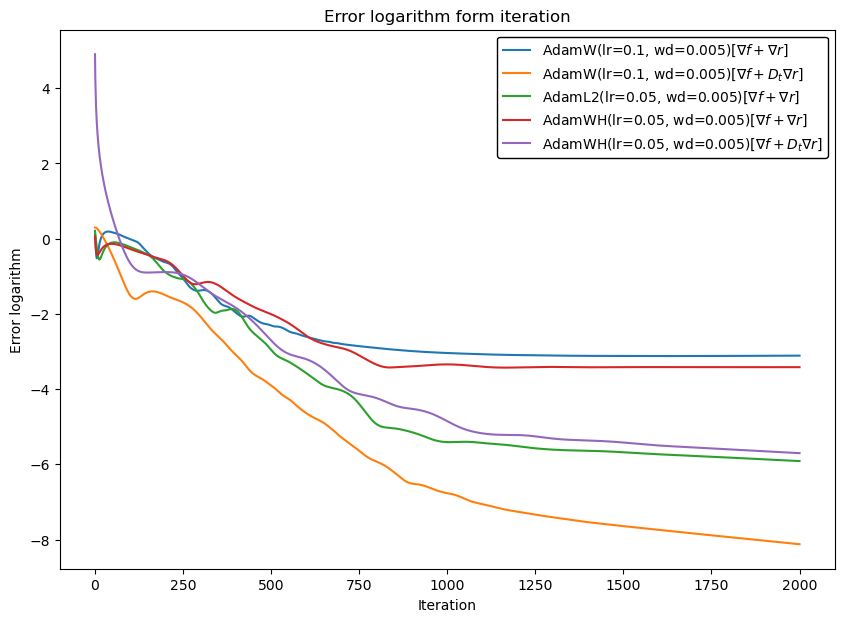
\includegraphics[width=\textwidth]{pictures/mushrooms/adams_error.png}
\caption{Adam on dataset mushrooms}
    \label{fig:adams_error}
\end{minipage}
\hfill
\begin{minipage}[h]{0.4\linewidth}
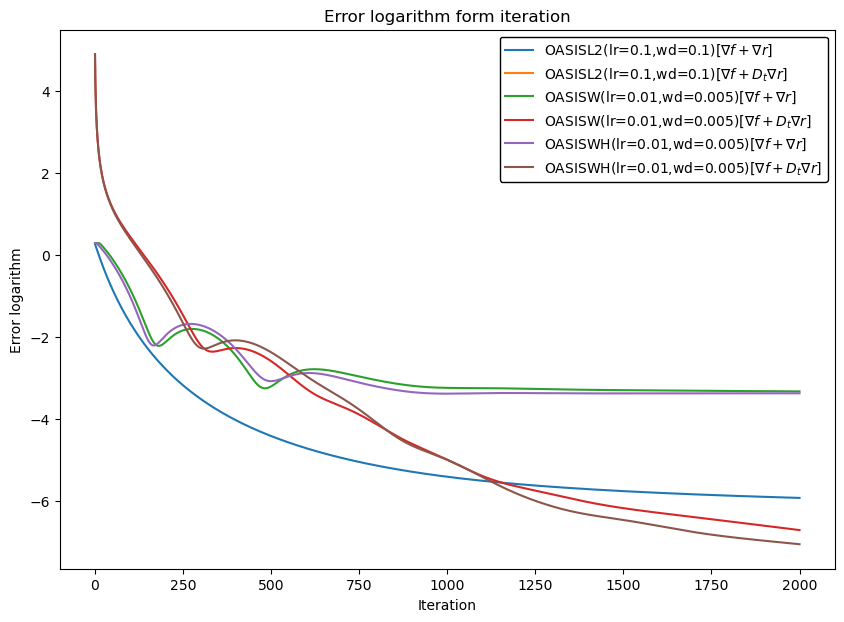
\includegraphics[width=\textwidth]{pictures/mushrooms/oasis_error.png}
    \caption{OASIS on dataset mushrooms}
        \label{fig:oasis_error}
\end{minipage}
\label{fig:oasis_error}
\end{figure}


\begin{figure}[H]
\centering
    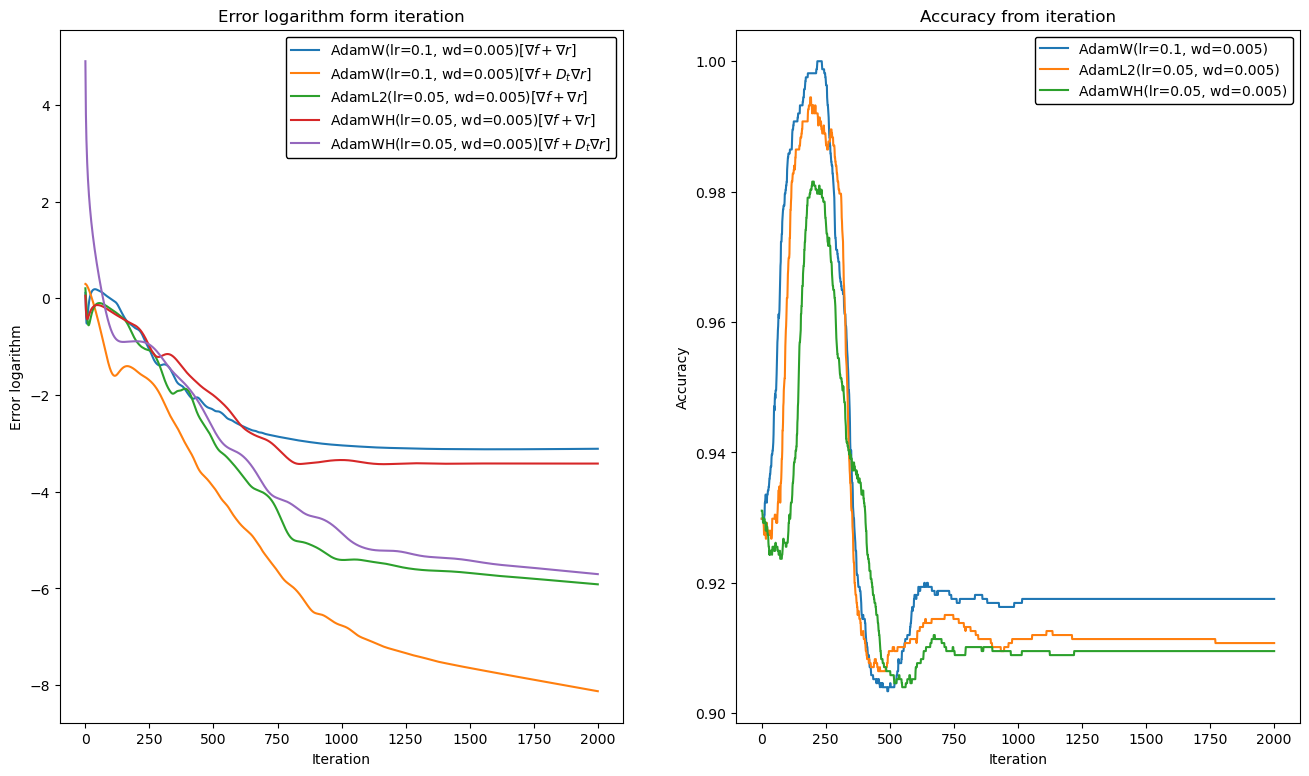
\includegraphics[width=0.7\textwidth]{pictures/mushrooms/main_adam.png}
    \caption{Adam algrorithms on dataset: mushrooms}
    \label{fig:main_mushrooms_adam}
\end{figure}

\begin{figure}[H]
\centering
    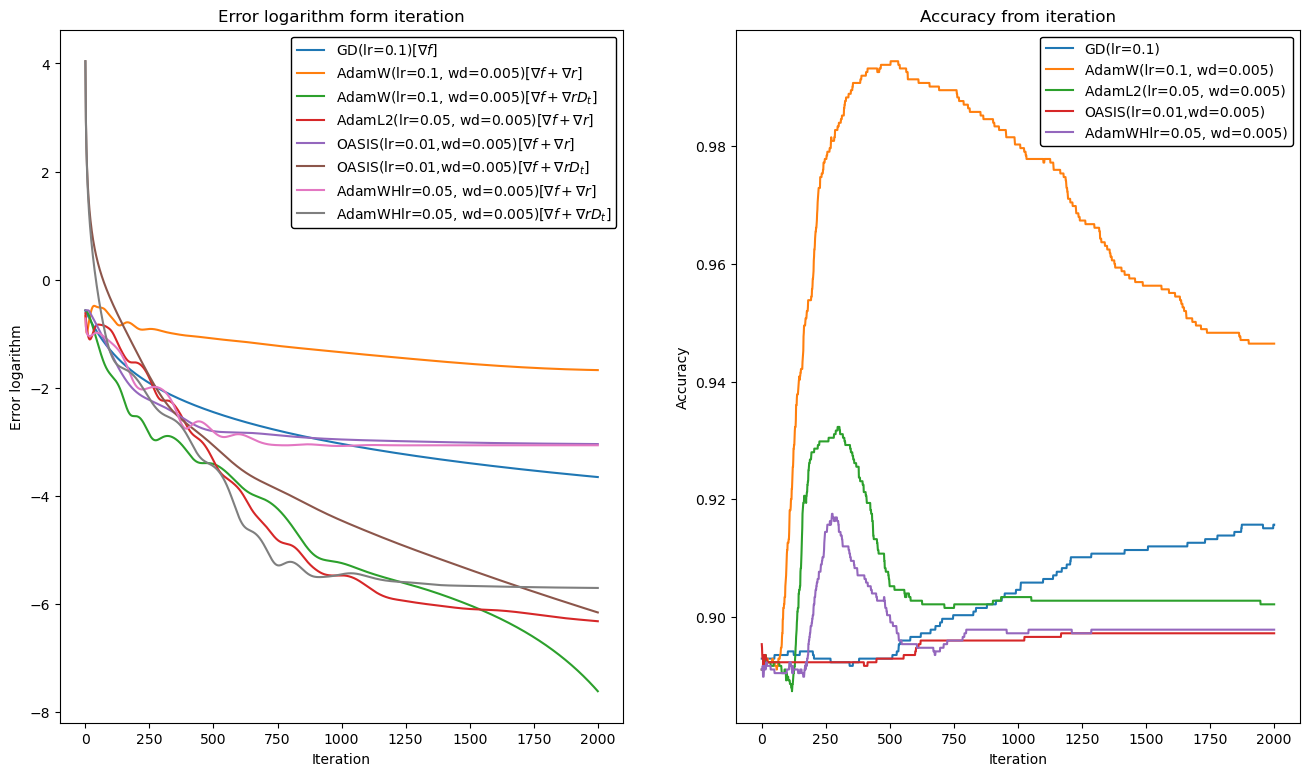
\includegraphics[width=0.7\textwidth]{pictures/mushrooms/main_mushrooms.png}
    \caption{Compare different optimization algorithms on dataset: mushrooms}
    \label{fig:main_mushrooms}
\end{figure}
As we can see, the AdamW method shows the best result compared to other optimization algorithms, it is also clear that the new AdamW criterion converges much faster than the old one, and thus it has a better generalization ability compared to other methods.

\begin{figure}[H]
\centering
    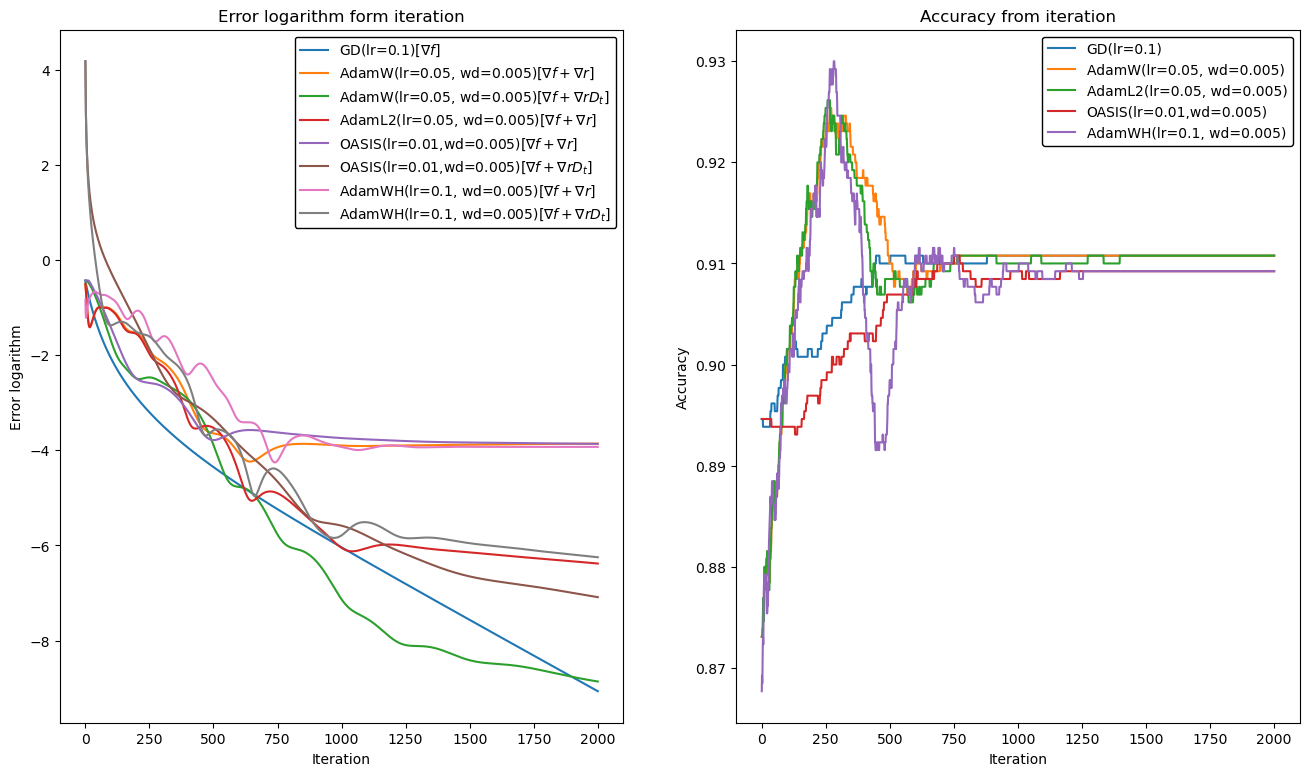
\includegraphics[width=0.7\textwidth]{pictures/wine/main_wine.png}
    \caption{Compare different optimization algorithms on dataset: mushrooms}
    
        \label{fig:main_wine}
\end{figure}
Here we see a similar picture as in the last example.
\subsubsection{Mushrooms}
Here are all the experiments that were performed on the mushrooms dataset. Learning rate and weight decay are signed for each method on the picture, as well as the criterion used to calculate the error.
\begin{figure}[h]
\begin{minipage}[h]{0.5\linewidth}
\center{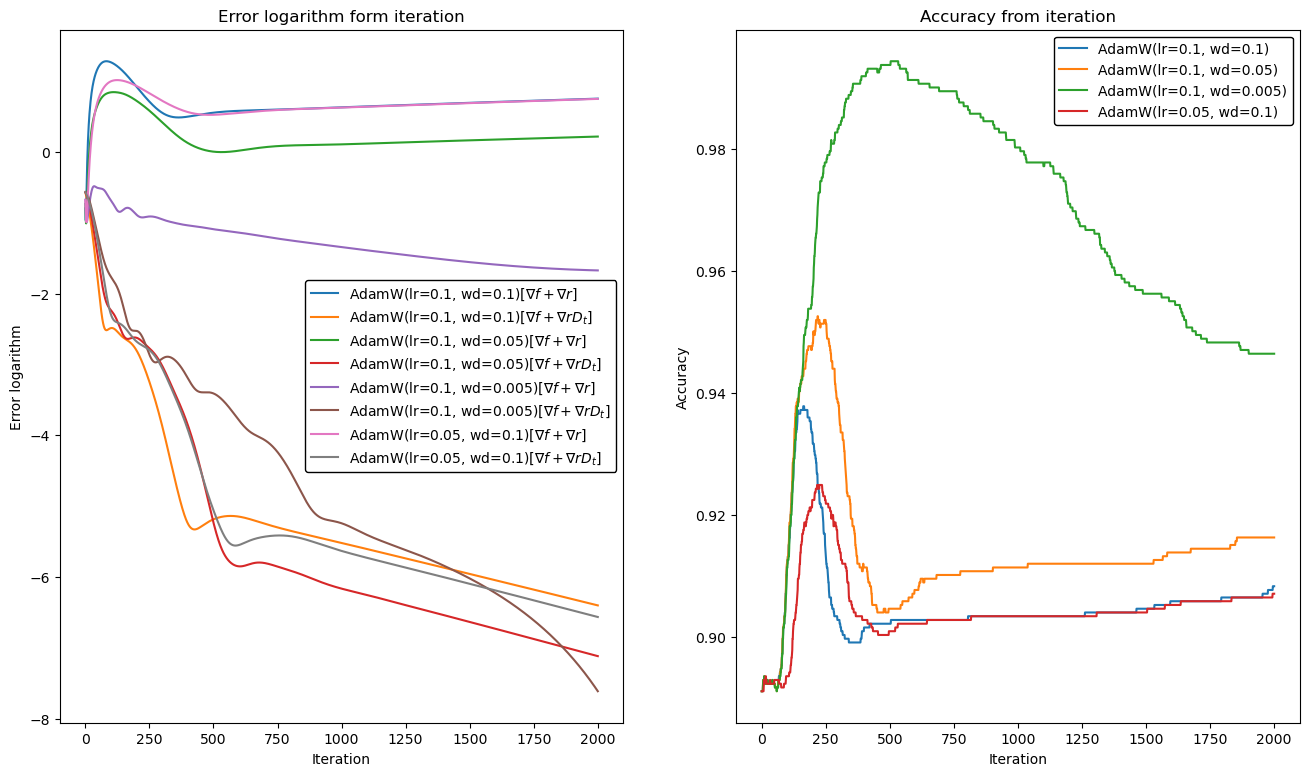
\includegraphics[width=\linewidth]{pictures/mushrooms/m_adamw_2000_1.png}}
\end{minipage}
\hfill
\begin{minipage}[h]{0.5\linewidth}
\center{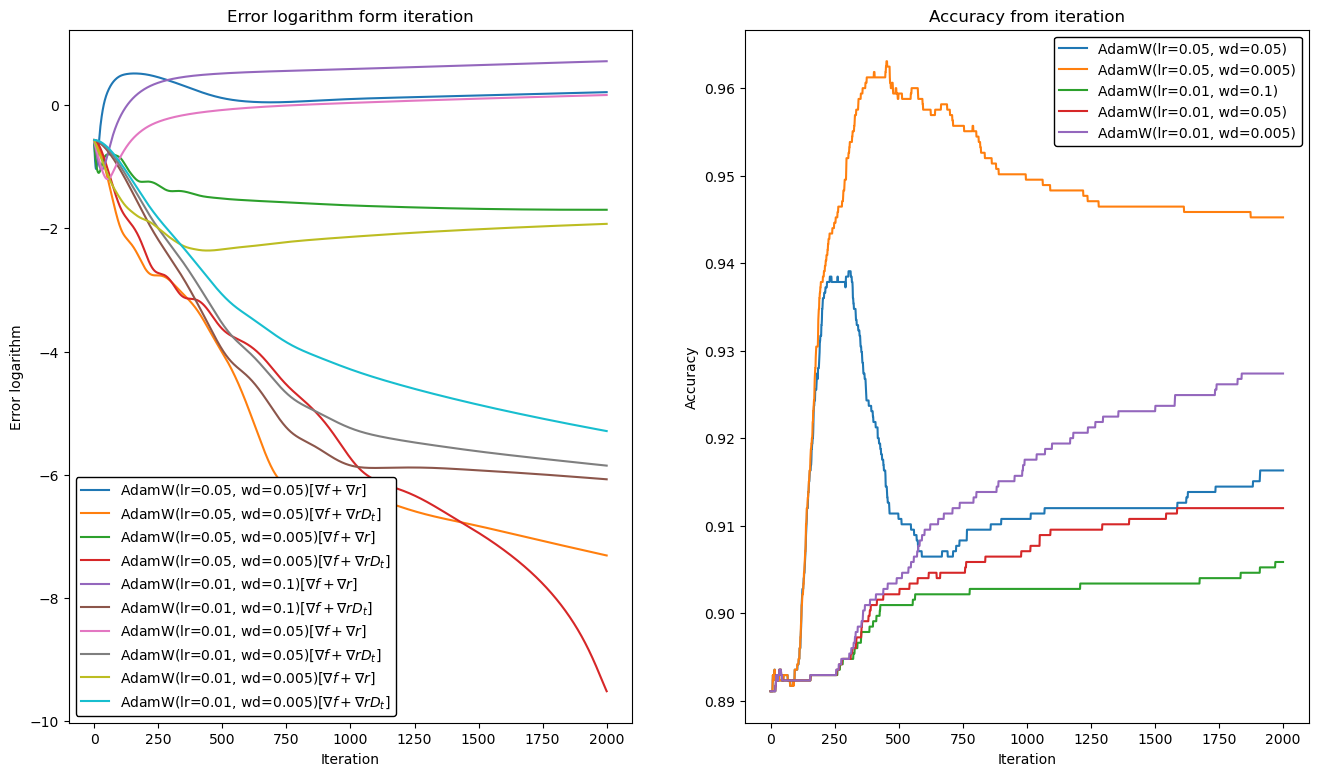
\includegraphics[width=\linewidth]{pictures/mushrooms/m_adamw_2000_2.png}}
\end{minipage}
\caption{AdamW on dataset mushrooms}

\label{fig:m_adamw}
\end{figure}

\begin{figure}[H]
\begin{minipage}[h]{0.5\linewidth}
\center{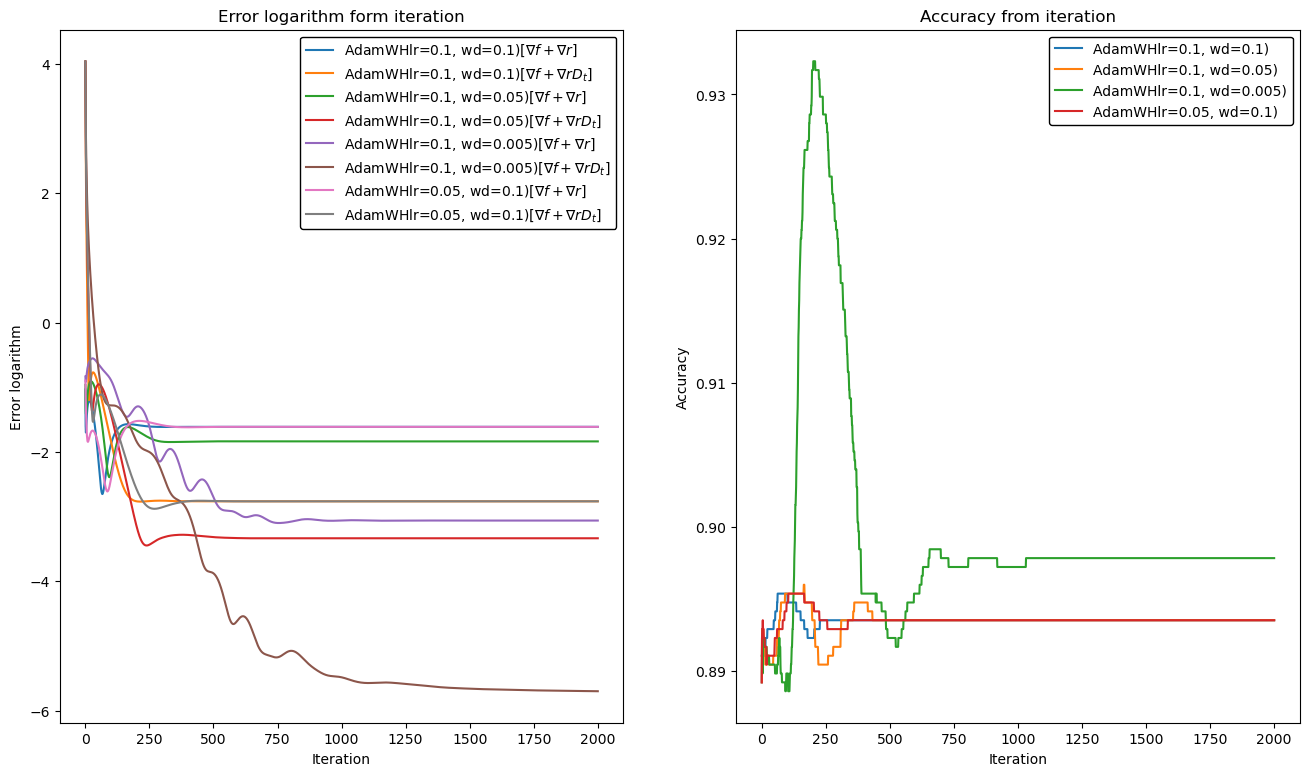
\includegraphics[width=\linewidth]{pictures/mushrooms/m_adamwh_2000_1.png}}
\end{minipage}
\hfill
\begin{minipage}[h]{0.5\linewidth}
\center{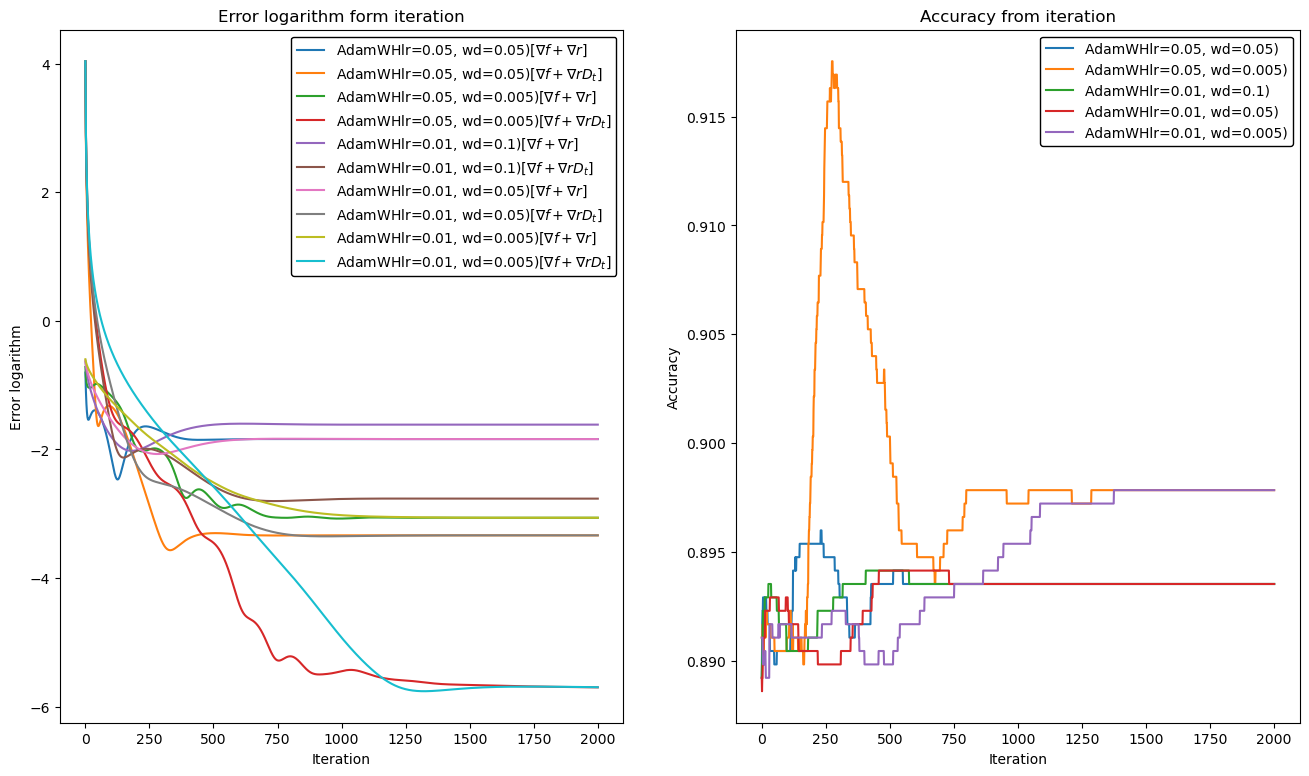
\includegraphics[width=\linewidth]{pictures/mushrooms/m_adamwh_2000_2.png}}
\end{minipage}
\caption{AdamWH on dataset mushrooms}
\label{fig:m_adamwh}
\end{figure}

\begin{figure}[H]
\begin{minipage}[h]{0.5\linewidth}
\center{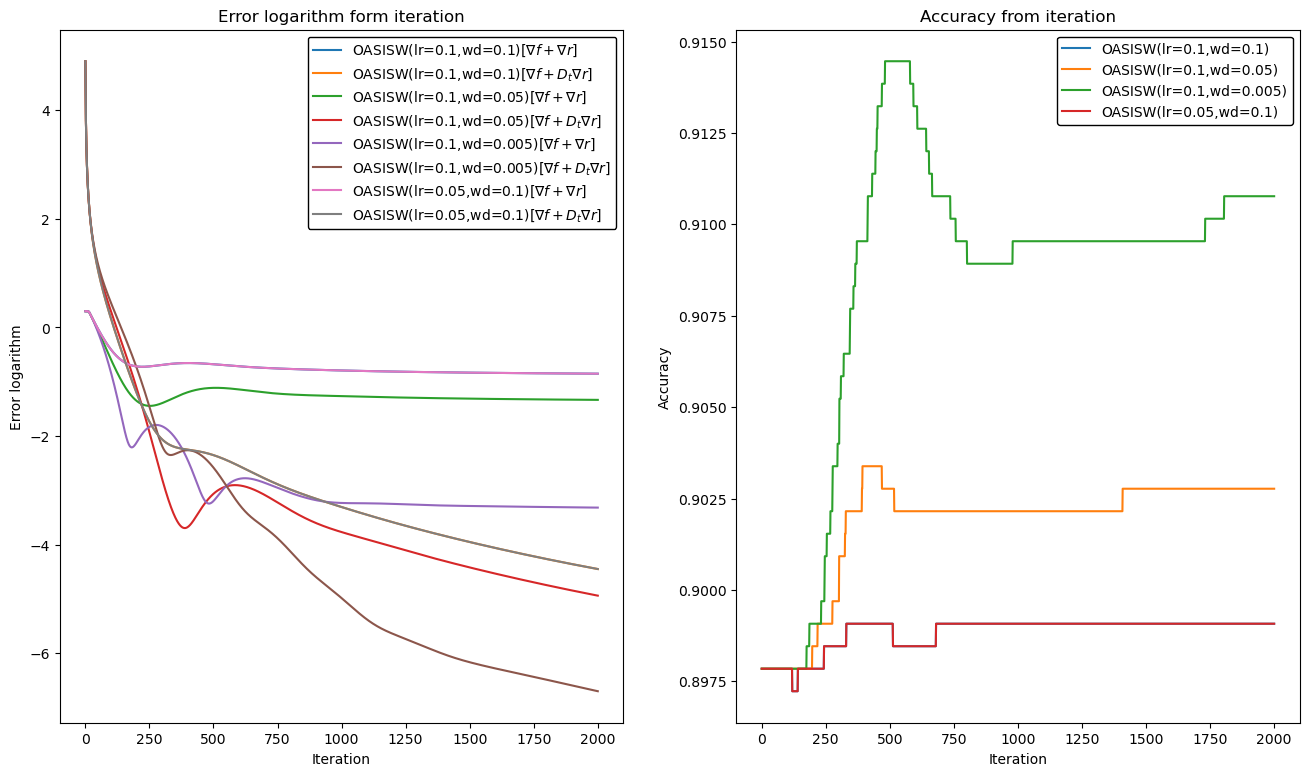
\includegraphics[width=\linewidth]{pictures/mushrooms/m_oasisw_1.png}}
\end{minipage}
\hfill
\begin{minipage}[h]{0.5\linewidth}
\center{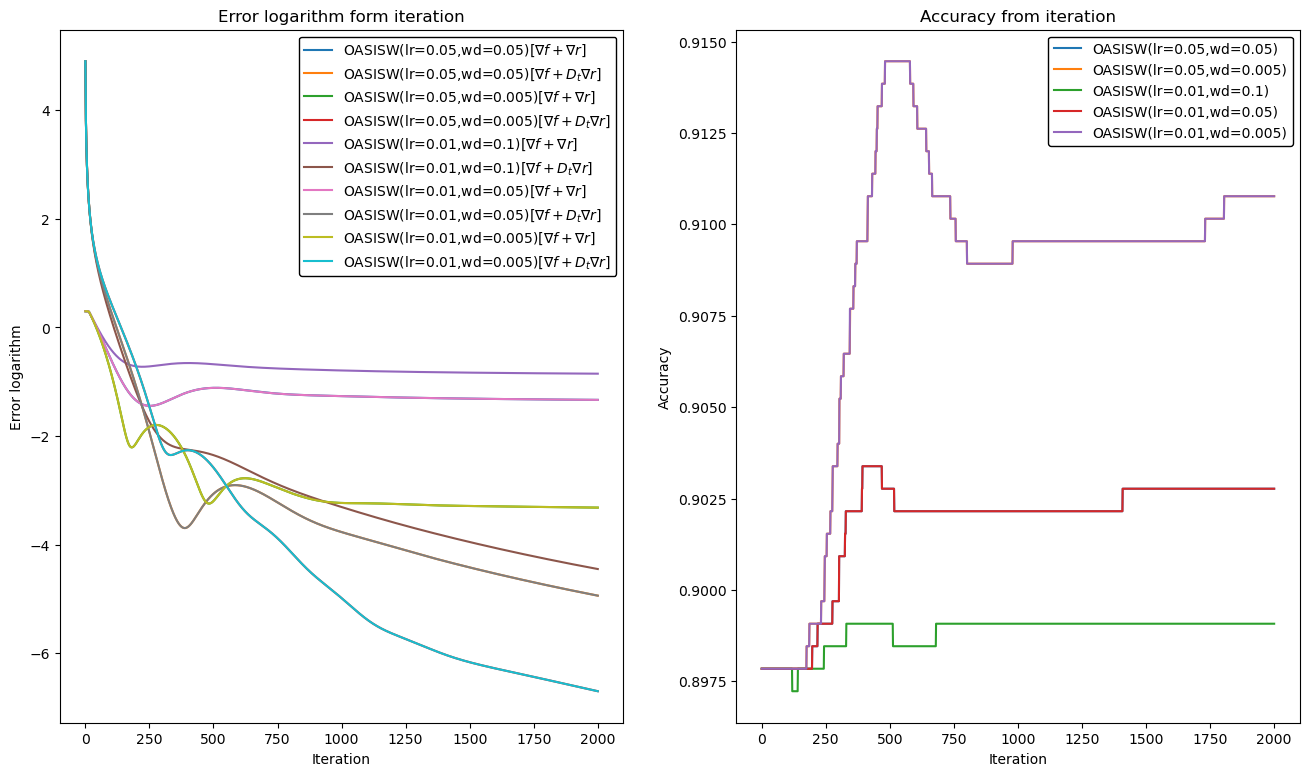
\includegraphics[width=\linewidth]{pictures/mushrooms/m_oasisw_2.png}}
\end{minipage}
\caption{OASISW on dataset mushrooms}
\label{fig:m_oasisw}
\end{figure}

\begin{figure}[H]
\begin{minipage}[h]{0.5\linewidth}
\center{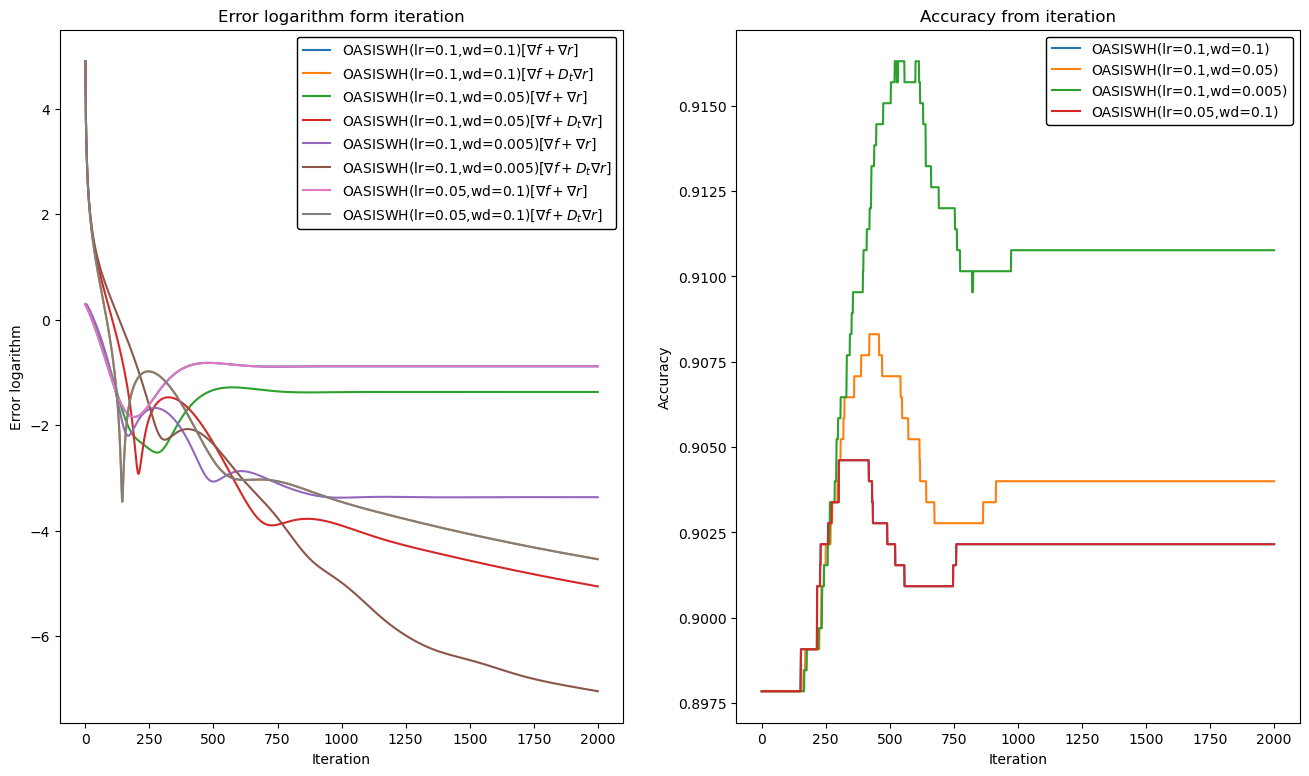
\includegraphics[width=\linewidth]{pictures/mushrooms/m_oasiswh_1.png}}
\end{minipage}
\hfill
\begin{minipage}[h]{0.5\linewidth}
\center{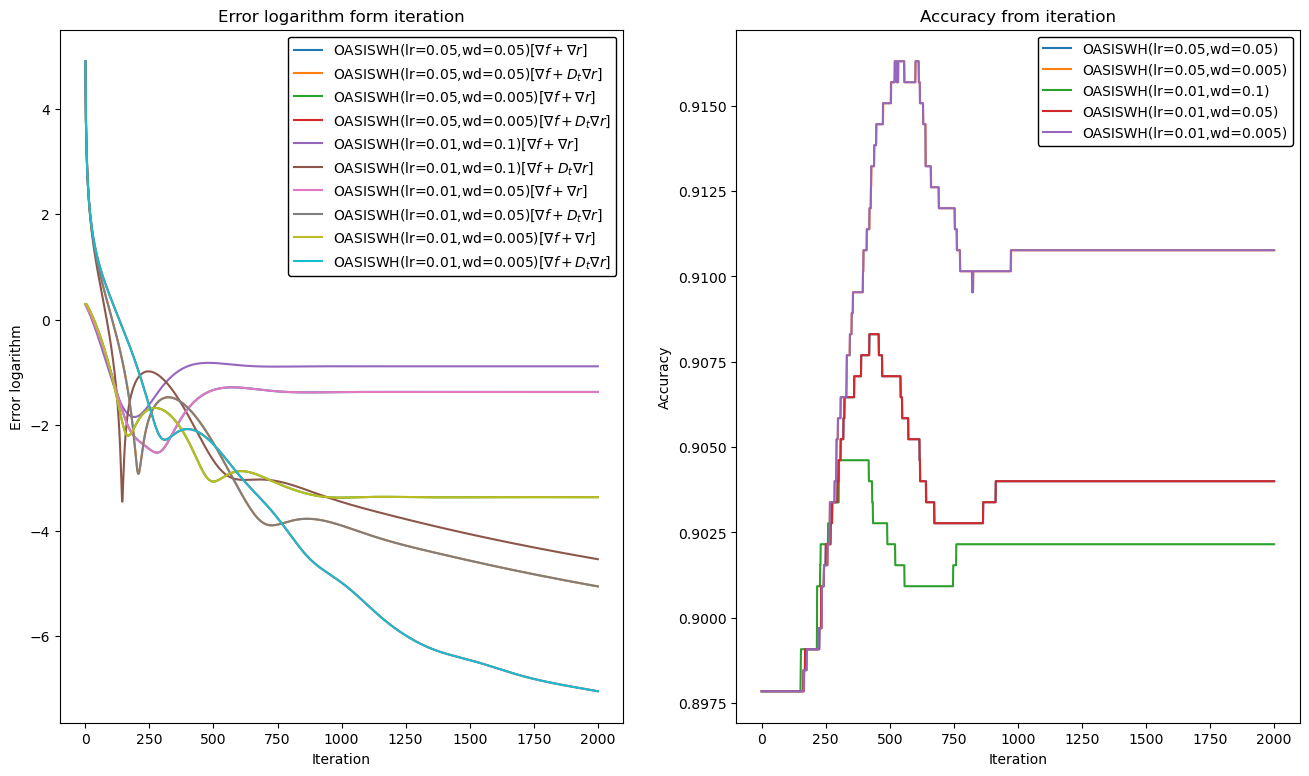
\includegraphics[width=\linewidth]{pictures/mushrooms/m_oasiswh_2.png}}
\end{minipage}
\caption{OASISWH on dataset mushrooms}
\label{fig:m_oasiswh}
\end{figure}


\begin{figure}[H]
\begin{minipage}[h]{0.5\linewidth}
\center{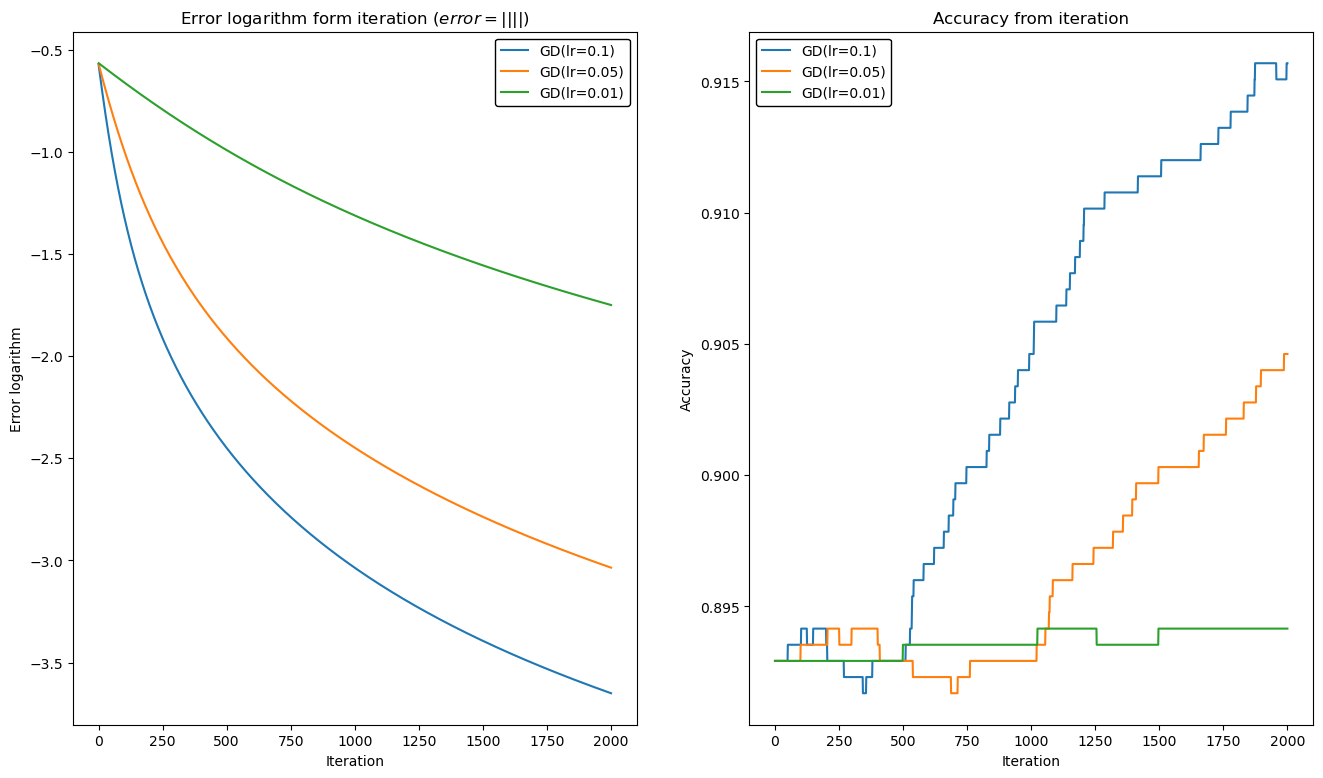
\includegraphics[width=\linewidth]{pictures/mushrooms/m_gd_2000.png}}
\end{minipage}
\hfill
\begin{minipage}[h]{0.5\linewidth}
\center{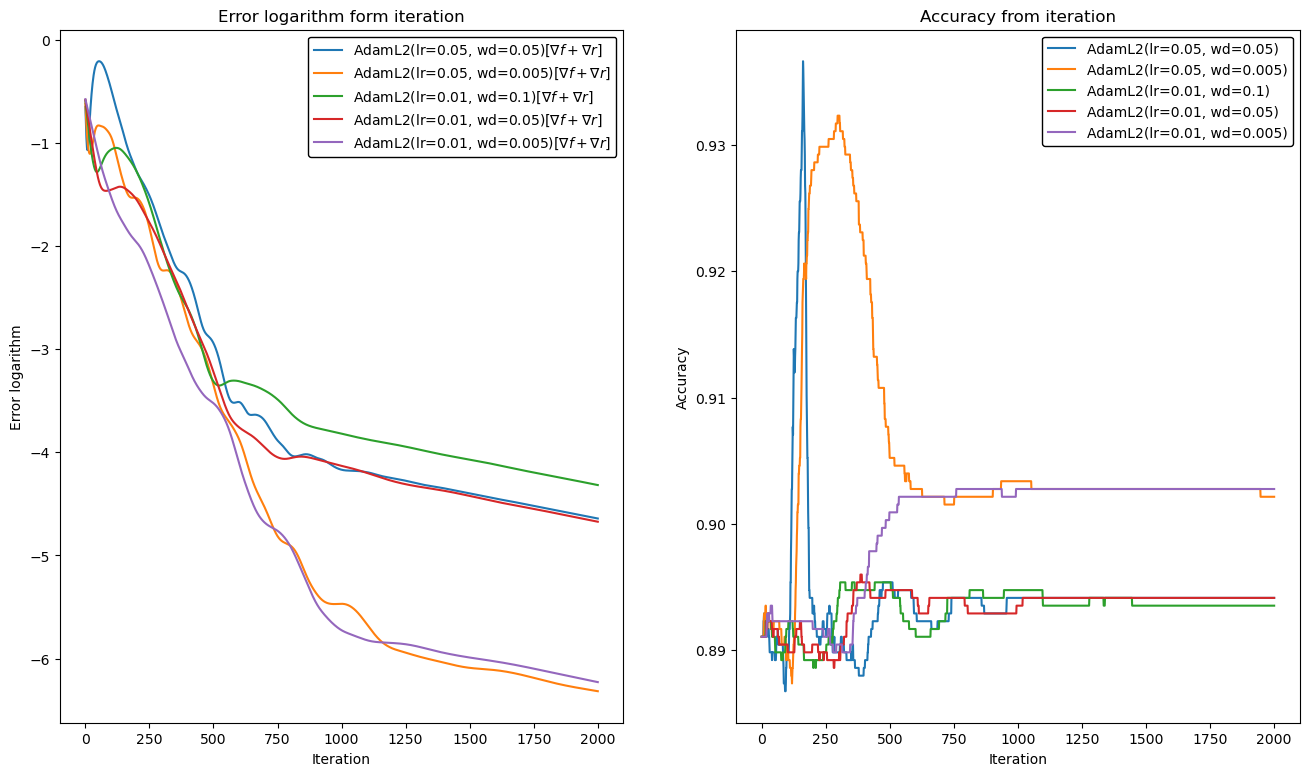
\includegraphics[width=\linewidth]{pictures/mushrooms/m_adaml2_2000.png}}
\end{minipage}
\caption{Gradient descent and AdamL2 on dataset mushrooms}
\label{fig:m_gd_adaml2}
\end{figure}

%xuy 
\subsubsection{Wine}
Here are all the experiments that were performed on the \href{https://archive.ics.uci.edu/ml/datasets/wine}{wine} dataset. Learning rate and weight decay are signed for each method on the picture, as well as the criterion used to calculate the error.
\begin{figure}[H]
\begin{minipage}[h]{0.5\linewidth}
\center{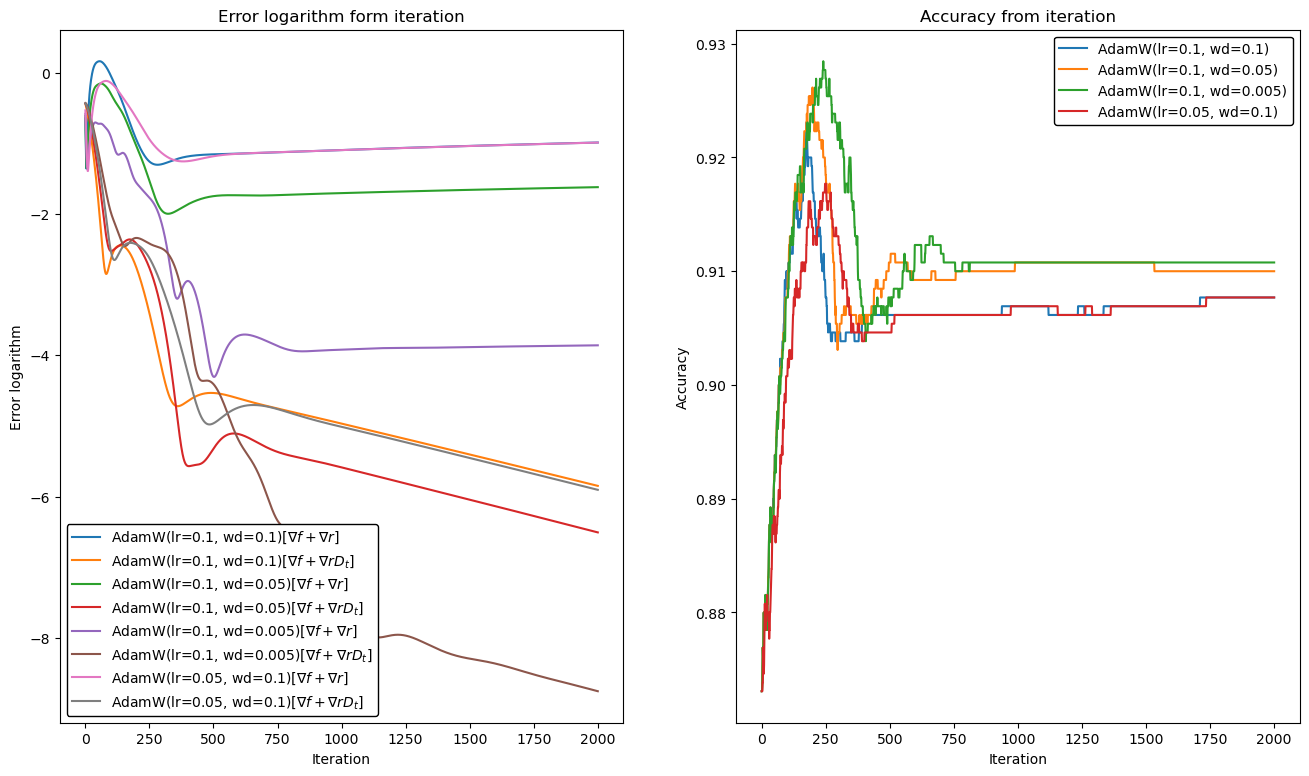
\includegraphics[width=\linewidth]{pictures/wine/w_adamw_2000_1.png}}
\end{minipage}
\hfill
\begin{minipage}[h]{0.5\linewidth}
\center{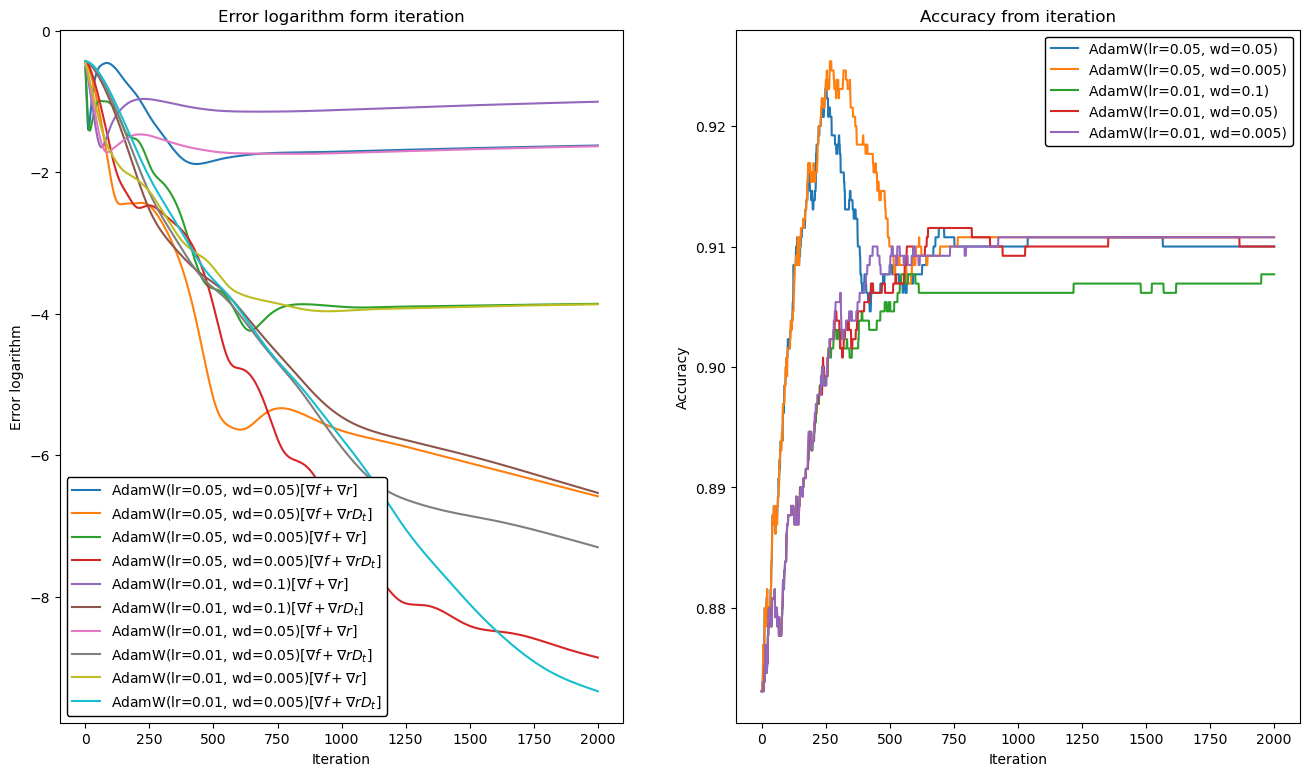
\includegraphics[width=\linewidth]{pictures/wine/w_adamw_2000_2.png}}
\end{minipage}
\caption{AdamW on dataset wine}

\label{fig:w_adamw}
\end{figure}

\begin{figure}[H]
\begin{minipage}[h]{0.5\linewidth}
\center{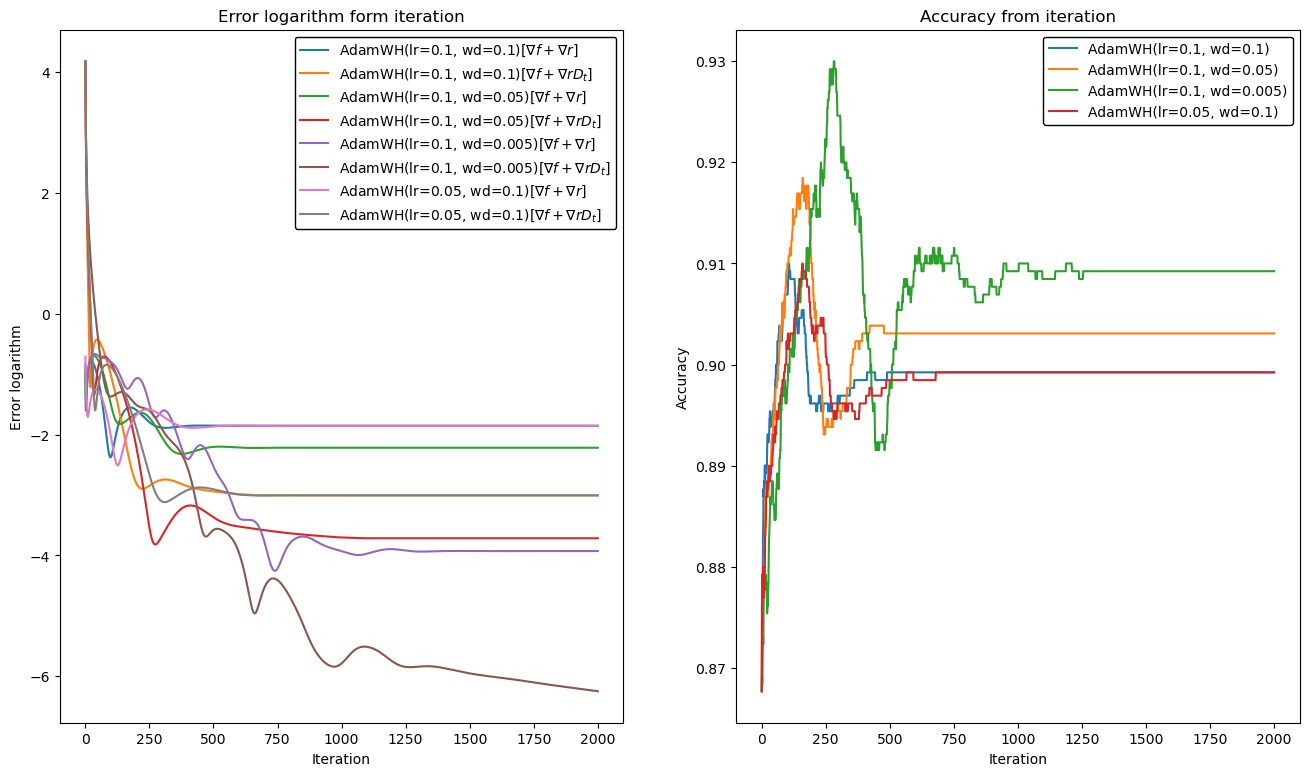
\includegraphics[width=\linewidth]{pictures/wine/w_adamwh_2000_1.png}}
\end{minipage}
\hfill
\begin{minipage}[h]{0.5\linewidth}
\center{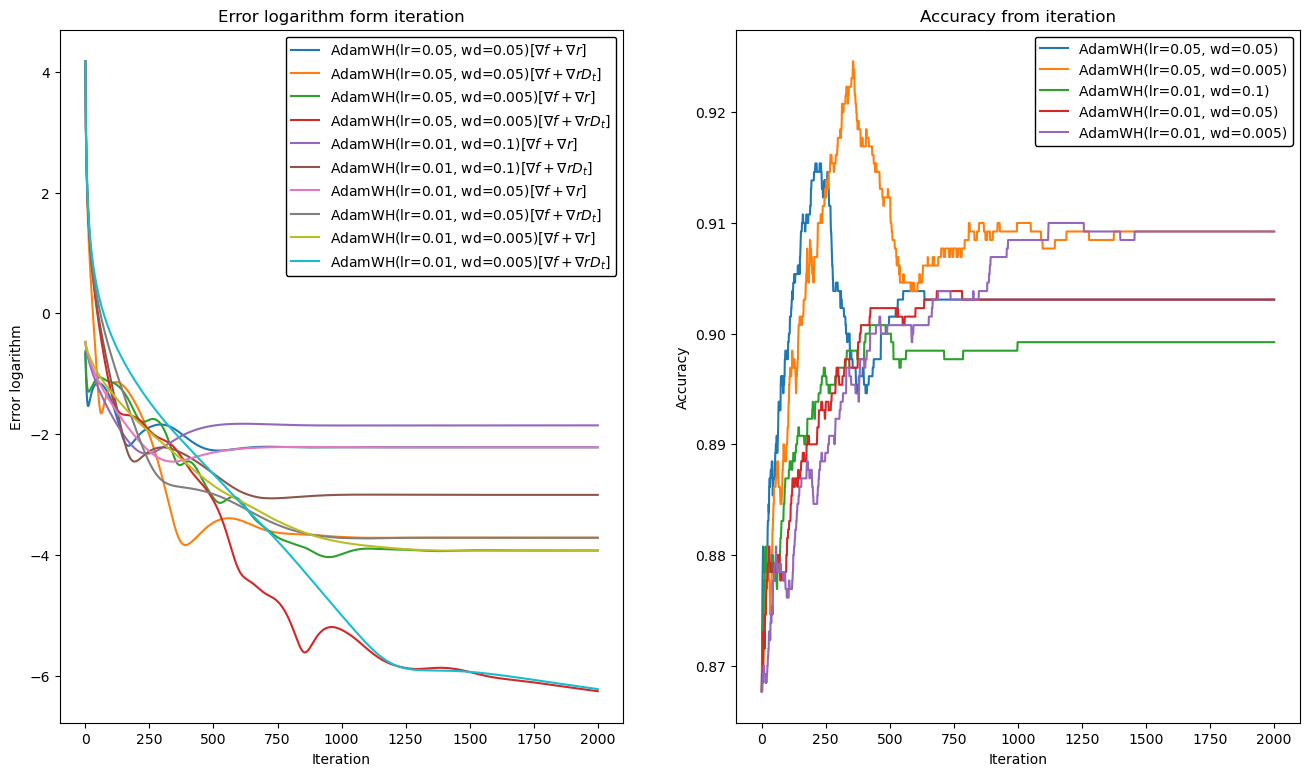
\includegraphics[width=\linewidth]{pictures/wine/w_adamwh_2000_2.png}}
\end{minipage}
\caption{AdamWH on dataset wine}
\label{fig:w_adamwh}
\end{figure}

\begin{figure}[H]
\begin{minipage}[h]{0.5\linewidth}
\center{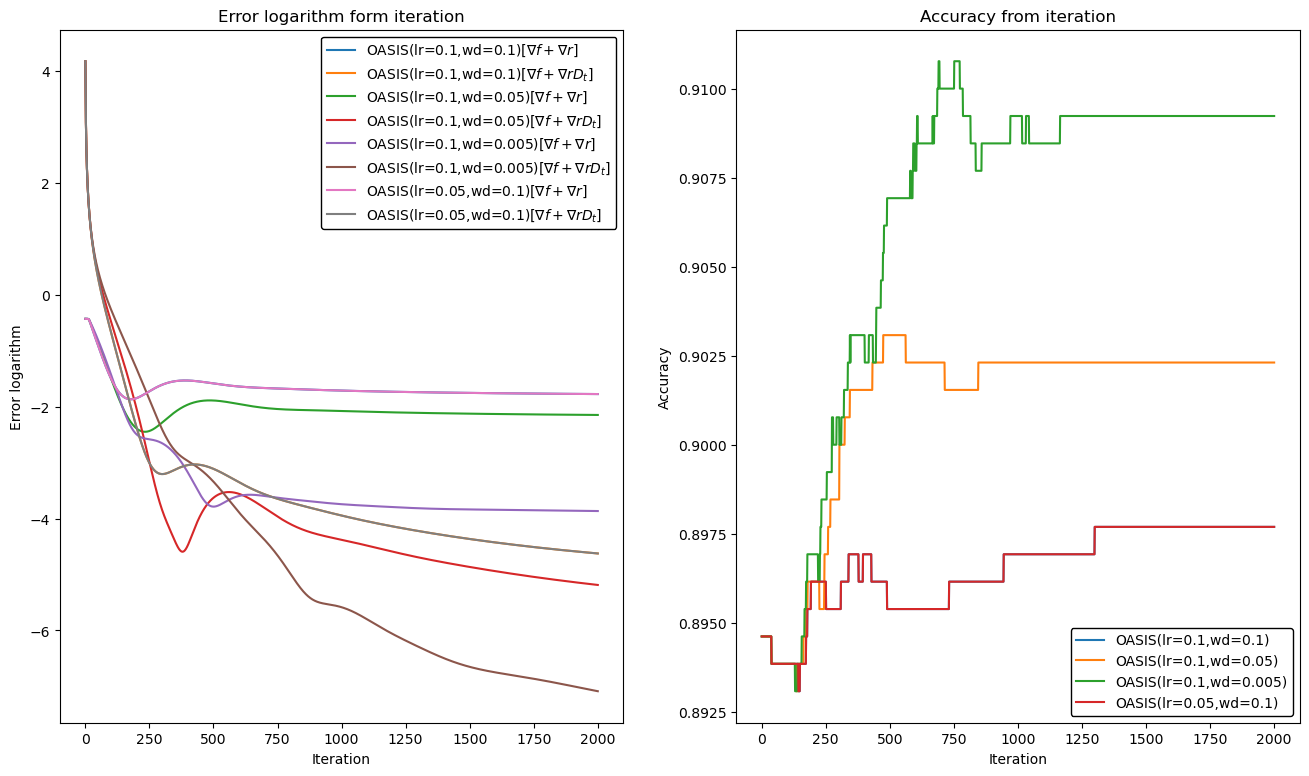
\includegraphics[width=\linewidth]{pictures/wine/w_oasis_2000_1.png}}
\end{minipage}
\hfill
\begin{minipage}[h]{0.5\linewidth}
\center{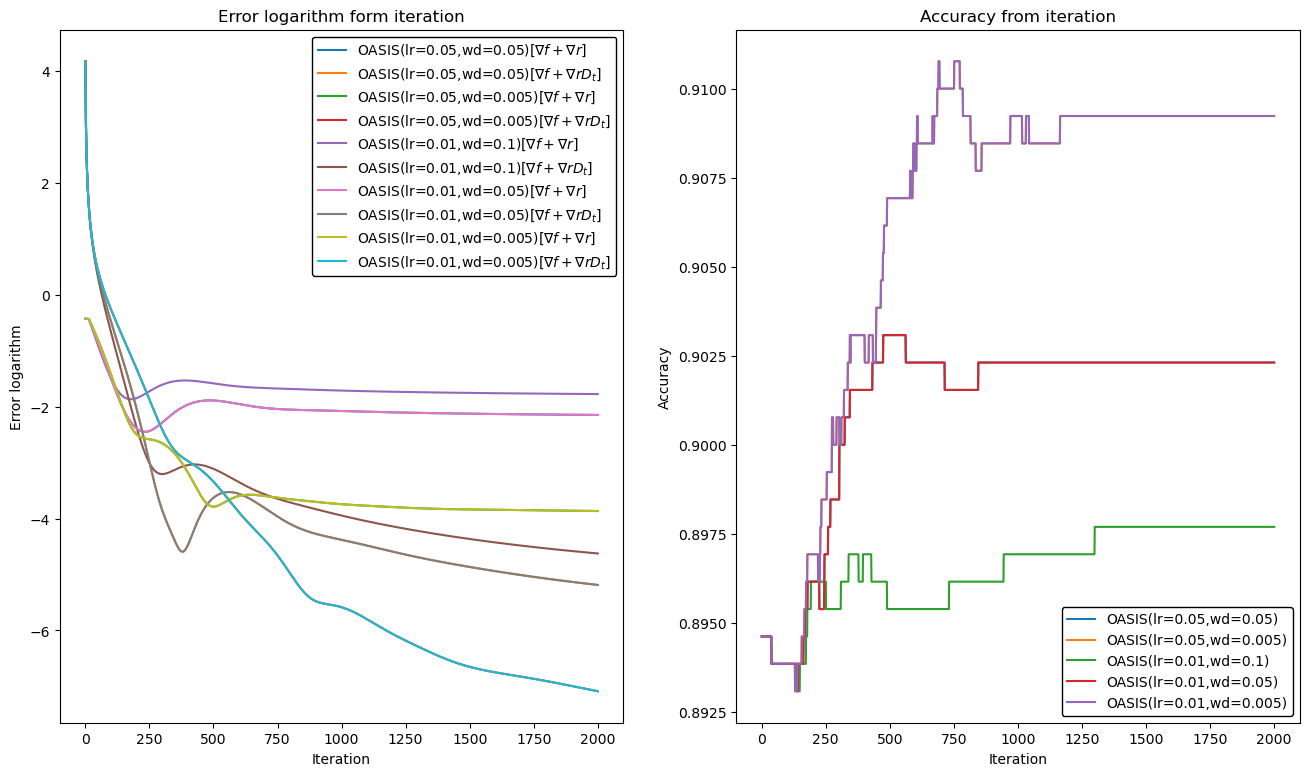
\includegraphics[width=\linewidth]{pictures/wine/w_oasis_2000_2.png}}
\end{minipage}
\caption{OASISW on dataset wine}
\label{fig:w_oasisw}
\end{figure}


\begin{figure}[H]
\begin{minipage}[h]{0.5\linewidth}
\center{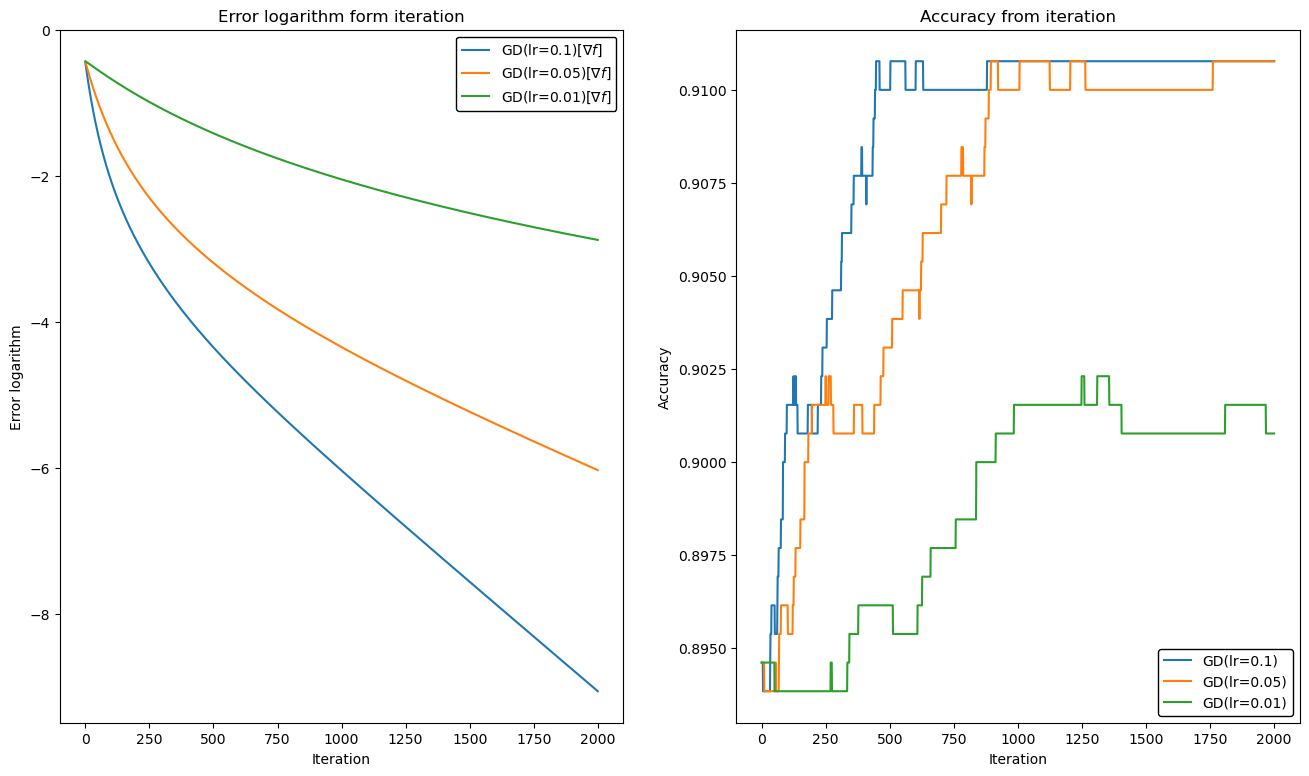
\includegraphics[width=\linewidth]{pictures/wine/w_gd_2000.png}}
\end{minipage}
\hfill
\begin{minipage}[h]{0.5\linewidth}
\center{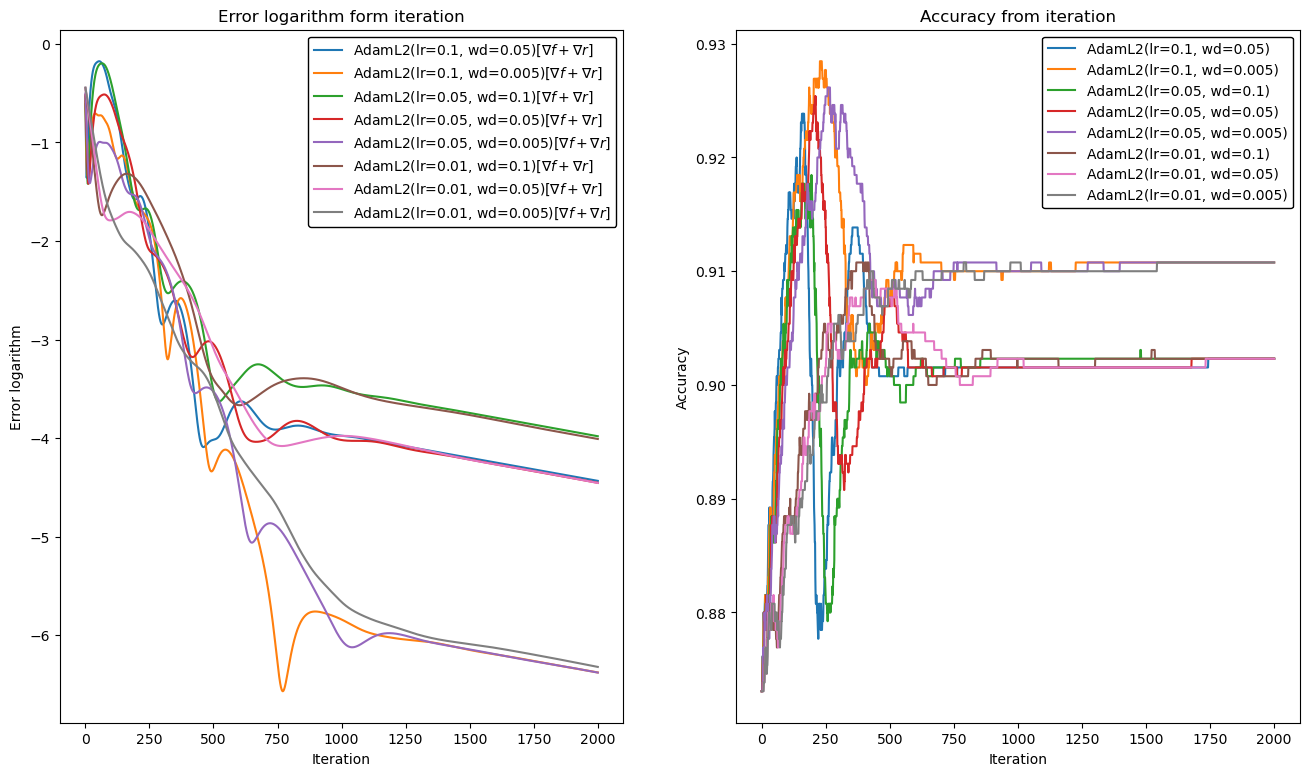
\includegraphics[width=\linewidth]{pictures/wine/w_adaml2_2000.png}}
\end{minipage}
\caption{Gradient descent and AdamL2 on dataset wine}
\label{fig:w_gd_adaml2}
\end{figure}

And to finalize our results let's show the results of training \href{https://pytorch.org/vision/main/models/generated/torchvision.models.resnet18.html}{ResNet18} on 4 different optimizators with \href{https://pytorch.org/docs/stable/generated/torch.optim.lr_scheduler.CosineAnnealingLR.html}{CosineAnnealingLr} on dataset \href{https://www.cs.toronto.edu/~kriz/cifar.html}{CIFAR10}.

\begin{figure}[H]
\centering
    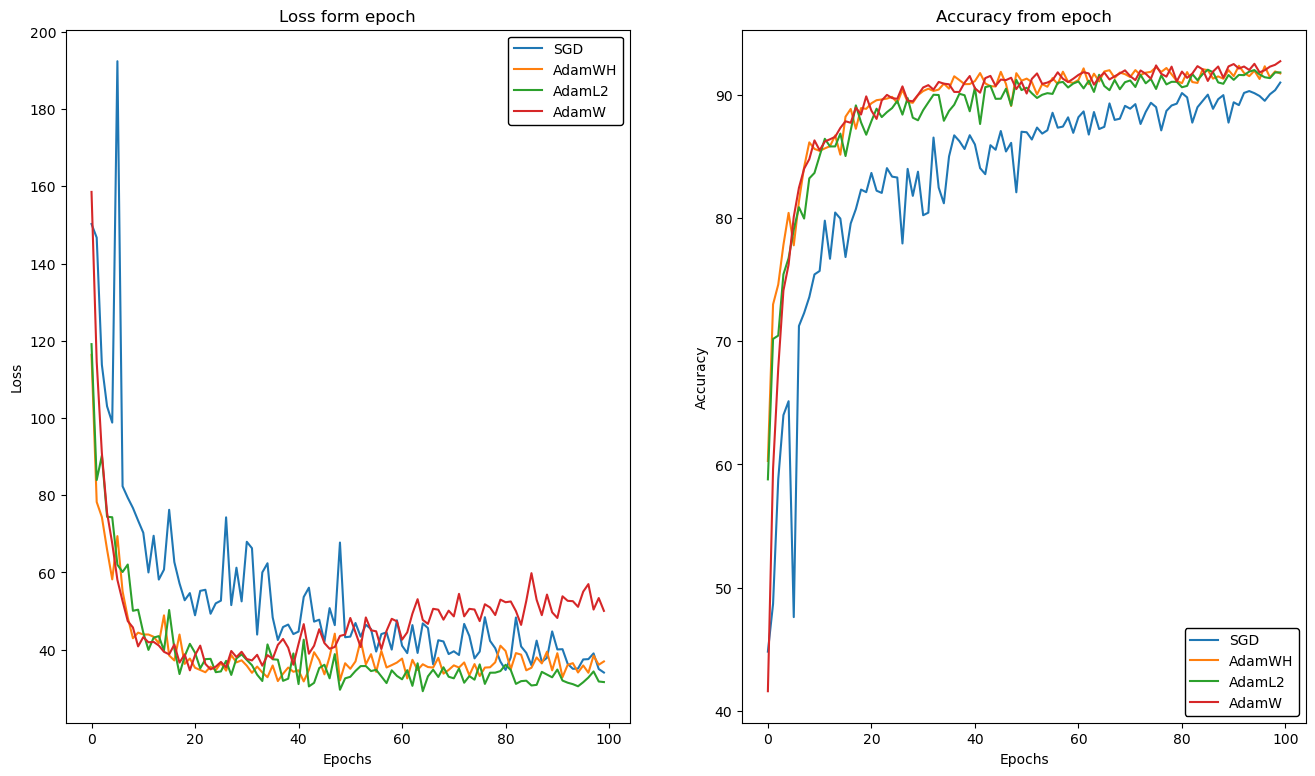
\includegraphics[width=0.7\textwidth]{pictures/nn_results.png}
    \caption{Compare different optimization algorithms on dataset: CIFAR10}

        \label{fig:main_resnet18}
\end{figure}
AdamW shows the worst results for the loss function, but wins all other methods in accuracy on the test sample, exactly this generalizing ability of the AdamW method was mentioned earlier.

\subsection{Conclusion:}
This paper investigated preconditioning methods with weight decay regularization. Two theorems were established for these methods, each under different assumptions regarding the target loss function. The theorems demonstrated that these methods converge to a different criterion that is significantly superior to the original one. Consequently, these methods exhibit reduced overfitting and greater generalization ability, leading to excellent performance when training neural networks. Empirical results were also presented to support these findings.


\bibliographystyle{unsrtnat}
\bibliography{refs}

\end{document}